%----------------------------------------------------------------------------------------
%	PACKAGES AND OTHER DOCUMENT CONFIGURATIONS
%----------------------------------------------------------------------------------------
\documentclass[11pt,fancychapters]{report}
\usepackage[a4paper, total={6in, 8in}]{geometry}
\usepackage{standalone}
\usepackage{listings}
\usepackage{color}
\usepackage{setspace}
\usepackage{hyperref}
\usepackage{acro}
\usepackage{amsmath}
\usepackage{amsthm}
\usepackage{graphicx}
\usepackage{geometry}
\usepackage{subcaption}
\usepackage{cancel}
\usepackage{tikz}
\usepackage{color}
\usetikzlibrary{calc,trees,positioning,arrows,chains,shapes.geometric,%
    decorations.pathreplacing,decorations.pathmorphing,shapes,%
    matrix,shapes.symbols}
\DeclareAcronym{nn}{
	short = NN,
	long = neural network
}

\DeclareAcronym{neta}{
	short = NETA,
	long = net-activation
}

\DeclareAcronym{mse}{
	short = MSE,
	long = mean square error
}

\DeclareAcronym{kNN}{
	short = kNN,
	long = k-nearest neighbor,
}

\DeclareAcronym{sgd}{
	short = SGD,
	long = stochastic gradient descent,
}


\DeclareAcronym{adam}{
	short = adam,
	long = adaptive moment estimation
}

\DeclareAcronym{cnn}{
	short = CNN,
	long = convolutionnal neural network
}

\DeclareAcronym{rnn}{
	short = RNN,
	long = recursive neural network
}
\definecolor{Code}{rgb}{0,0,0}
\definecolor{Decorators}{rgb}{0.5,0.5,0.5}
\definecolor{Numbers}{rgb}{0.5,0,0}
\definecolor{MatchingBrackets}{rgb}{0.25,0.5,0.5}
\definecolor{Keywords}{rgb}{0,0,1}
\definecolor{self}{rgb}{0,0,0}
\definecolor{Strings}{rgb}{0,0.63,0}
\definecolor{Comments}{rgb}{0,0.63,1}
\definecolor{Backquotes}{rgb}{0,0,0}
\definecolor{Classname}{rgb}{0,0,0}
\definecolor{FunctionName}{rgb}{0,0,.7}
\definecolor{Operators}{rgb}{0,0,0}
\definecolor{Background}{rgb}{0.98,0.98,0.98}

\lstdefinestyle{python}{
  numbers=left,
  numberstyle=\footnotesize,
  numbersep=1em,
  xleftmargin=1em,
  framextopmargin=2em,
  framexbottommargin=2em,
  showspaces=false,
  showtabs=false,
  showstringspaces=false,
  frame=l,
  tabsize=4,
  % Basic
  basicstyle=\ttfamily\small\setstretch{1},
  backgroundcolor=\color{Background},
  language=Python,
  % Comments
  commentstyle=\color{Comments}\slshape,
  % Strings
  stringstyle=\color{Strings},
  morecomment=[s][\color{Strings}]{"""}{"""},
  morecomment=[s][\color{Strings}]{'''}{'''},
  % keywords
  morekeywords={import,from,class,def,for,while,if,is,in,elif,else,not,and,or,print,break,continue,return,True,False,None,access,as,,del,except,exec,finally,global,import,lambda,pass,print,raise,try,assert},
  keywordstyle={\color{Keywords}\bfseries},
  % additional keywords
  morekeywords={[2]@invariant},
  keywordstyle={[2]\color{Decorators}\slshape},
  emph={self},
  emphstyle={\color{self}\slshape},
  breaklines=true
}

\geometry{top=1.3in,bottom=1.3in}
\hypersetup{
    colorlinks,
    citecolor=black,
    filecolor=black,
    linkcolor=black,
    urlcolor=black
}

\definecolor{DarkerGreen}{RGB}{0,179,45}

\newtheorem{exmp}{Example}[section]

\newcommand{\codeExample}[2]{
	\begin{exmp}
      #1
      \noindent\begin{minipage}{\linewidth}
      \begin{lstlisting}[style=python]
          #2
      \end{lstlisting}
      \end{minipage}
    \end{exmp}
}

\newcommand\MyLBrace[2]{%
  \left.\rule{0pt}{#1}\right\}\text{#2}}
  
%----------------------------------------------------------------------------------------
%	REPORT
%----------------------------------------------------------------------------------------

\title{ARN_PW3}

\begin{document}

%%%%%%%%%%%%%%%%%%%%%%%%%%%%%%%%%%%%%%%%%
% Uppsala University Assignment Title Page 
% LaTeX Template
% Version 1.0 (27/12/12)
%
% This template has been downloaded from:
% http://www.LaTeXTemplates.com
%
% Original author:
% WikiBooks (http://en.wikibooks.org/wiki/LaTeX/Title_Creation)
% Modified by Olivier D'Ancona to fit HEIG-VD
% License:
% CC BY-NC-SA 3.0 (http://creativecommons.org/licenses/by-nc-sa/3.0/)

%\title{Title page with logo}
%----------------------------------------------------------------------------------------
%	PACKAGES AND OTHER DOCUMENT CONFIGURATIONS
%----------------------------------------------------------------------------------------

\documentclass[12pt]{article}
\usepackage[english]{babel}
\usepackage[utf8x]{inputenc}
\usepackage{amsmath}
\usepackage{graphicx}
\usepackage{float}
\usepackage[colorinlistoftodos]{todonotes}

\begin{document}

\begin{titlepage}

\newcommand{\HRule}{\rule{\linewidth}{0.5mm}} % Defines a new command for the horizontal lines, change thickness here

\center % Center everything on the page
 
%----------------------------------------------------------------------------------------
%	HEADING SECTIONS
%----------------------------------------------------------------------------------------

\textsc{\LARGE Haute École d'Ingénierie et de Gestion du Canton de Vaud}\\[1.5cm] % Name of your university/college

\includegraphics[scale=.2]{images/heig.png}\\[1cm] % Include a department/university logo - this will require the graphicx package
\textsc{\Large Gestion de projet de Machine Learning}\\[0.5cm] % Major heading such as course name
\textsc{\large GML}\\[0.5cm] % Minor heading such as course title


%----------------------------------------------------------------------------------------
%	TITLE SECTION
%----------------------------------------------------------------------------------------

\HRule \\[0.4cm]
{ \huge \bfseries Crapauduc - 2022}\\[0.4cm] % Title of your document
\HRule \\[1.5cm]
 
%----------------------------------------------------------------------------------------
%	AUTHOR SECTION
%----------------------------------------------------------------------------------------

\begin{minipage}{0.4\textwidth}
\begin{flushleft} \large
\emph{Authors:}\\
Schaller \textsc{Joris}\\ % Your name
D'Ancona \textsc{Olivier}\\ % Your name
Logan  \textsc{Victoria}\\ % Your name
Akoumba \textsc{Erica Ludivine}\\ % Your name
Wichoud \textsc{Nicolas}\\ % Your name

\end{flushleft}

\end{minipage}\\[1.5cm]

% If you don't want a supervisor, uncomment the two lines below and remove the section above
%\Large \emph{Author:}\\
%John \textsc{Smith}\\[3cm] % Your name

%----------------------------------------------------------------------------------------
%	DATE SECTION
%----------------------------------------------------------------------------------------

{\large \today}\\[2cm] % Date, change the \today to a set date if you want to be precise

\vfill % Fill the rest of the page with whitespace

\end{titlepage}


\end{document}

\newpage
\pagenumbering{roman}
\tableofcontents
\newpage
\pagenumbering{arabic}

\chapter{Introduction}
\paragraph*{}
Ce projet de machine learning nous a été proposé dans le cadre du cours de Gestion et valorisation de projet en Machine Learning (GML), donné au cours du cinquième semestre du cursus de Bachelor en Informatique et système de communication orienté ingénierie des données à la HEIG-VD. Le but de ce travail est de nous faire découvrir la gestion et organisation impliquée par un travail de machine learning, autant au niveau de la recherche technologique qu'au niveau de l'organisation d'équipe, notamment au niveau de la distribution de tâches, gestion d'équipe et de délais. \newline

Le projet décrit ici est un projet existant ayant déjà été réalisé plusieurs fois par le professeur et de précédents étudiant.e.s : l'étude de crapauducs. Un crapauduc est un “petit conduit sous une route, permettant le passage protégé des batraciens” - selon Le Robert. En 2017, dix-huit crapauducs ont étés construits le long de la route d'Aubonne à Gimel - canton de Vaud - afin de permettre aux grenouilles, crapauds et tritons de traverser la route des bois à l'étang en toute sécurité. L'image \ref{fig:Un des 18 crapauducs installés pour l'étude} montre l'un de ceux qui ont été installés. \newline

À l'intérieur de ces crapauducs ont été installée une caméra équipée d'un capteur, qui implique la prise d'une petite série de photos (\textit{Figure \ref{fig:Exemples des images d'amphibiens prises par les cameras}}) lors de la détection de mouvement, ainsi qu'une planche afin de faciliter la distinction des objets du sol. Comptant moins de caméras que de crapauducs, les caméras n'étaient pas rattachée à un crapauduc et comptent donc des images prises depuis différents crapauducs.\newline

\begin{figure}[!htb]
    \centering
    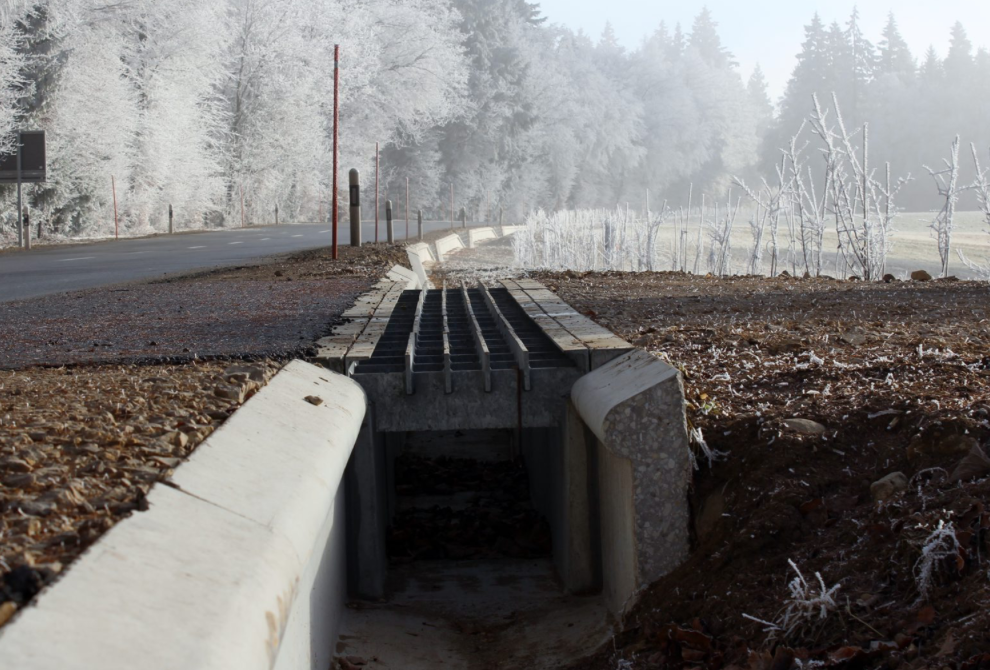
\includegraphics[width=200px]{images/introduction_crapauduc_exterieur.png}
    \caption{Un des 18 crapauducs installés pour l'étude}
    \label{fig:Un des 18 crapauducs installés pour l'étude}
\end{figure}

\newpage

\begin{figure}[!htb]
    \centering
    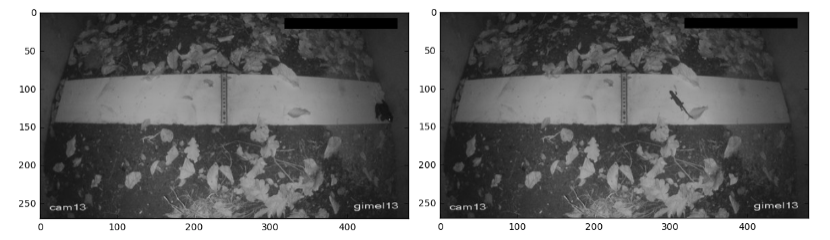
\includegraphics[width=300px]{images/introduction_crapauduc_exemple_prise_camera.png}
    \caption{Exemples des images d'amphibiens prises par les cameras}
    \label{fig:Exemples des images d'amphibiens prises par les cameras}
\end{figure}

Au terme de la première année d'utilisation, ces voies ont été empruntées par plus de 6'000 crapauds, grenouilles et tritons confondus. Ce comptage a été effectué par des chercheurs, qui ont du regarder les images prises par les caméras et compter les animaux "à la main". Le projet Crapauduc vise ainsi à utiliser l'apprentissage automatique (Machine Learning) pour automatiser le comptage des batraciens. \newline

Notre objectif pour ce projet est donc de détecter la présence ou non de grenouille/crapaud et tritons (en considérant les grenouilles et crapauds comme une seule et même catégorie) en utilisant l'apprentissage automatique, ce afin de déterminer si la constructions de ces crapauducs est efficace. Pour se faire, nous avons les prises des caméras du 23 février 2017 au 20 avril de la même année, totalisant près de 1 million d'images, dont on connaît pour chacune la caméra dont elle provient ainsi que le moment où la photo a été prise (date, heure, minute et seconde).\newline

Enfin, le professeur Satizabal Mejia Hector Fabio nous a également mis à disposition sa labelisation pour certaines images, des bounding box pour certaines également, ainsi que les données météos enregistrées durant cette période (notamment la température, le vent, la précipitation et l'humidité).



\chapter{Outils}

\paragraph*{But}

Nous avons constitué un repository GitHub contenant des scripts permettant de transformer les données brutes en données utilisables pour l'analyse. Ces scripts sont disponibles dans le repository utils sur GitHub.

\section{Colabeler}

Afin de réaliser les bounding boxs et les labels, nous avons utilisé le logiciel Colabeler, permettant d'annoter les images pour l'object detection. Ainsi, nous pouvons ajouter des bounding box facilement et rapidement. Il a été utilisé dans le cadre de la création du filtre de la planche et dans la constitution de l'ensemble de données de test.

\section{Conversion de format}

Nous avons écrit plusieurs petit scripts Python permettant de convertir les labels en différents formats. Il existe plusieurs manières de définir les bounding boxs. Elles peuvent être définies comme un point d'ancrage et une taille plus une hauteur ou simplement comme deux points. De plus, il existe différentes nomenclatures pour stocker ces images, telles que le format coco stocké dans un fichier .json qui est associé au dataset COCO. Il se peut que les données soient encore stockées sous forme d'un csv ou d'un fichier manifest qui peut être utile pour des services comme Amazon Sagemaker. Ainsi, nous avons créé plusieurs fonctions de conversion de csv à json, de xml à csv, ou encore de pascalvoc à csv, afin de pouvoir annoter les images avec l'outil colabeler.

\section{Comptage des labels}

Un petit script a été élaboré afin de compter les labels déjà effectués, ce qui permet d'avoir une liste des images déjà traitées et de constituer un sous-ensemble rapidement pour entraîner des algorithmes.

\section{Folder Shortener}

Ce script bash permet de simplifier le chemin d'accès aux images, pour une question de clarté et d'entretien du projet. Les chemins d'accès sont ainsi plus courts et plus lisibles, ce qui bénéficie à la compréhension du projet.

\section{Fusion des dataframes}

Nous avons également un script permettant de fusionner plusieurs fichier csv en un seul, ce qui permet de constituer un ensemble de données plus important afin de réaliser des analyses complètes. Par exemple, alors que les dossiers étaient partitionnés, notre fichier d'analyse regroupe ainsi tous les dossiers.

\section{Tri des images}

Nous avons également un script bash qui permet à partir d'une liste de fichier de déplacer tous les fichiers en une seule fois. Ainsi il est possible d'exporter un subset rapidement à partir d'une liste.

\section{Réorganisation des données}

Le script d'unnesting a permis de transformer la structure des données. Au début, la structure était partitionnée par caméra et par date, ce qui facilitait la navigation mais compliquait la gestion des fichiers. Ainsi, nous avons utilisé ce script pour changer le partitionnement uniquement par caméra, ce qui permet de gérer une arborescente moins profonde et regrouper le travail. De plus, ce script stocke les nouveaux résultats dans un csv ce qui permet de faire des analyses sur tout le dataset.

\chapter{Gestion du projet}
\section{Organisation du projet}
Dès le départ, nous avons décider de travailler avec git, plus précisement 
en utilisant le site \url{https://github.com}. Nous avons donc créé une organisation afin de séparer les différents dépots. Nous en avons définis 2, mais les membres de l'organisation étaient libres d'en ajouté d'autres.
\begin{itemize}
    \item crapauduc.  Ce dépôt est le dépot principal où les notebooks des modèles sont déposés, nous y avons aussi placé les rapports des anciens étudiants afin d'y avoir un accès rapide. Nous y avons aussi déposé un subset d'image d'environ 0.5 Gib permettant le fine tuning.
    \item utils. Ce dépôt contient des scripts faisant des transformormations ou des analyses sur les données. Nous y avons par exemple un script qui permet de convertir les annotations de csv à COCO.
\end{itemize}

De plus, nous avons créer un compte google ayant le doux nom de \verb|student GML| afin d'avoir un espace google drive de 15 GiB pour stocker les données ainsi qu'une intégration facilitée dans le service \url{colab.research.google.com} de Google. Nous croyions être prêts.


\section{Gestion du temps de travail}
Dès le départ, nous avons décider de travailler à distance afin de dédier 
la totalité de la journée à ce projet sans perdre de temps dans les transports publiques. En effet, le mardi où tombe le cours de GML, nous n'avons pas d'autre cours que ce dernier. Ainsi, un mardi typique se déroule comme suit:
\begin{itemize}
    \item 8h00 - 13h15: Libre, mais souvent on prépare la séance de l'après-midi.
    \item 13h15 - 15h: Appel Teams, où nous expliquons notre avancement, normalement les différents problèmes rencontrés durant la semaine doivent être réglé avant la réunion. Planification des tâches pour la prochaine semaine, et répartition des tâches. Durant chaque réunion un membre du groupe prend des notes afin d'avoir un historique des discussions, ce procès verbale des réunions est stocké sur le google drive de \verb|student GML|.
    \label{item:seance}
\end{itemize}
La séance du mardi se résume donc essentiellement à un partage d'information entre les différents groupes de travail composé de 1 à 3 étudiant.e.s. Le travail proprement dit est pour la plupart effectué en dehors des réunions, soit le mardi après la réunion soit à un autre moment choisis par les membres du groupe.

\section{Gestion des tâches et répartition}
Nous avons poussé notre utilisation de github, en gérant nos tâches à l'aide de l'outil de gestion de projet \href{https://github.com/topics/kanban}{kanban} directement intégré dans github. Ainsi, nous pouvons savoir à n'importe quel moment quel membre de l'équipe travail sur quelle partie du projet. De plus, nous pouvons voir les tâches en cours, les tâches terminées, les tâches en attentes, etc. 

\begin{figure}[htb!]
    \centering
    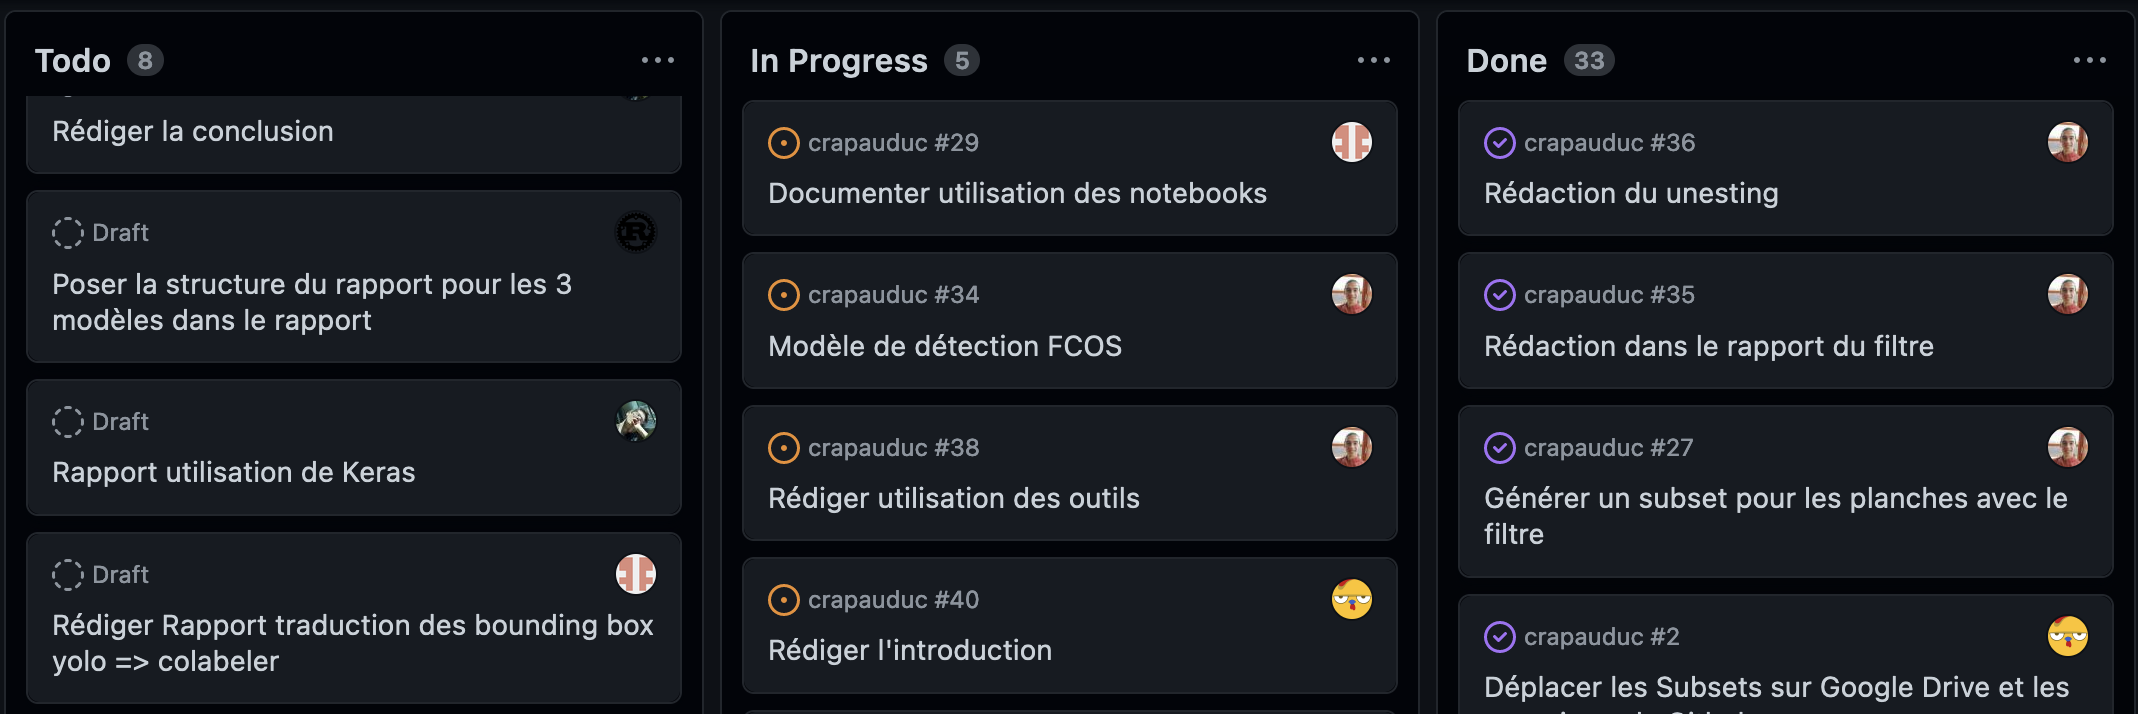
\includegraphics[width=0.8\linewidth]{images/kanban.png}
    \caption{Nos tâches du Kanban réparties en 3 catégories : à faire, en cours et terminées.}
    \label{fig:kanban}
\end{figure}

\paragraph{Problèmes d'organisation:} Nous avons décidé de ne pas élire de responsable au seins des étudiants. Cette décision a bien fonctionné pour certains aspects du travail, comme par exemple: la prise des notes durant les réunions.
Cependant les appels Teams étaient généralement coordonés par Olivier et Joris sans vraiment que cela ait été prévu. Ce n'était pas voulu puisque nous souhaitions une organisation horizontale, mais cette manière de fonctionner s'est imposé naturellement et nous avons gardé cette organisation pour la suite. Par coordination nous entendons de manière générale animer la discussion et amorcer les points suivants. 
L'organisation de travail à elle aussi subit des changements au cours du projet. Au début, nous avons travaillé de manière très individuelle sur les petites tâches initiales. Nous souhaitions pouvoir travailler de manière très parallèle et ce choix semblait être bon.
Néanmoins, cela nous a fait par la suite rencontrer deux nouveaux problèmes:
\begin{enumerate}
    \item Friction lors de la communication. \label{item:friction}
    \item Tâches trop complexes pour une seule personne. \label{item:complex}
\end{enumerate}
Notre organisation initiale fonctionnait bien au début du projet puisque nous avions beaucoup de petites tâches et nous avons bien avancé. 
Cependant, les tâches devenants de plus en plus grosses, les réunions ont pris de plus en plus de temps. 
En effet, nous avons rencontré beaucoup de problèmes qui étaient difficiles à résoudre seul, nous en discutions donc durant les réunions, et celles-ci commençait à prendre trop de temps.
Après quelques séances peu efficaces, nous avons réalisé qu'il serait plus judicieux de travail en petits groupes afin qu'une partie de la communication se fasse déjà entre les membres du sous-groupe et ainsi que l'on réduise les informations à partager lors des réunions. De plus travailler à plusieurs permettait de surmonter les problèmes rencontrés plus facilement.
\paragraph{}

Un point que nous remarquons après ce travail et le suivant : nous avons souvent débloquer des problèmes en les abandonnant puis en y revenant plus tard, ceci nous a permis d'aborder le problème une seconde fois avec de nouvelles connaissances qui nous ont fait avoir une deuxième approche différente de la première.
\\
Avec notre organisation actuelle, c'est à dire une réunion par semaine, nous n'arrivions pas forcément bien à laisser quelques jours le problème pour y revenir à tête reposée. Nous pensons que faire des réunions moins régulièrement, toutes les deux semaines par exemple, permettrait d'avoir plus de temps et ainsi de retravailler plusieurs fois le même problème entre deux réunions. Cependant cette solution demande des membres du groupe une plus grande autonomie, néanmoins en alliant cette proposition avec les petits groupes de travail présentés précédemment nous pensons que ça peut donner de bons résultats.

\paragraph{}
Un autre problème qui nous a embêté sur tout le projet et spécialement la fin du projet est le manque de ressources. Nous avons commencé par travailler en local, sur nos propres machines. Cependant, nous sommes très vite passés à Atlas afin de pouvoir héberger l'entièreté des données (500GiB) proche des notebooks. Atlas est une machine fournie par les professeurs sur laquelle un serveur Jupyter tournait. Cependant, nous n'avions pas accès à git depuis cet ordinateur ce qui posait des problèmes pour garder le projet synchronisé entre nos ordinateurs, github et Atlas. De plus, une fois les différentes analyses préliminaires terminées, il n'était absolument pas suffisant pour faire un entrainment d'un modèle comme DETR (60+ millions de paramètres). Nous avons donc migré sur l'offre gratuite de Google Colab. Les entrainements nécessitants toujours plusieurs dizaines de minutes, nous avons décider de payer Colab Pro afin d'avoir accès a des GPUs premiums 
et de pouvoir tester et fine tuner rapidement des modèles. Nous avons donc entrainé plusieurs modèles sur Colab Pro, et les avons évalués avec le benchmark COCO, ceci est expliqué plus en détail dans le chapitre \ref{chap:Evaluation}. Le soucis est le suivant, en ayant déplacé le projet sur plusieurs infrastructures, nous avons eu un projet éparpillé où il était dur de retrouver la dernière version. Un autre point notable est le manque de crédit à la fin du projet ce qui nous a empêcher de faire certaines analyses. En effet, DETR est tellement gros qu'il ne peut pas être chargé en mémoire sur un GPU non premium. Ainsi certaines expériences que nous aurions voulu réaliser n'ont pas été faites par manque de moyens. Nous voulions par exemple réaliser une centaine de prédictions sur un nouveau set et faire une fonction qui permet de filtrer certaines prédictions.
\paragraph{} En conclusion, nous sommes satisfait de l'organisation et du déroulement de ce projet, tous les membres du groupe ont travaillé sur des parties diverses et variées du projet. Tout le monde a ainsi pu expérimenter avec au moins un modèle de machine learning. De plus, la gestion s'est faite de manière naturelle et a permis de garder une bonne entente entre les différents étudiants même durant les moments où nous rencontrions des problèmes. Nous sommes particulièrement fière d'avoir su adapté notre organisation au cours du projet, afin de le mener à bien et ce malgrés notre manque de connaissance évident dans le domaine.
\chapter{Préparation des données}

\section{Acquisition des données}

\paragraph*{Problème} Lors de ce projet, les données doivent être accessible à tous les membres et doivent être stockées de manière uniformisée pour faciliter le travail de groupe. Nous avons alors opté pour une structure regroupant les images par caméra ; le nom de fichier correspondant est la date ISO standardisée de la date de la prise du fichier.

\paragraph*{Source} Nous avons récupéré un disque dur comprenant les 500GB dans le bureau de nos professeurs. La structure de fichier était partitionnée par caméra, année, jour, heure, minute. Cette structure était pratique pour naviguer dans les dossiers mais posait un problème pour extraire les informations car les métadonnées étaient stockées dans le chemin du fichier et non dans un fichier .csv externe. La nouvelle structure partitionnée par caméra permet d'avoir toutes les images regroupées et ainsi d'avoir les métadonnées au même endroit. Nous avons ainsi écrit des scripts de transformations que l'on peut trouver dans le repository `utils` sur GitHub.

\paragraph*{Format} Les images sont au format JPEG et sont toutes de la même taille, soit 1920x1080 pixels.

\paragraph*{Numéro de séquence} Une information qui n'était pas présente originellement était le numéro de séquence des images. Lorsque la caméra détectait un mouvement continu, la même action pouvait résulter en plusieurs images différentes. Nous avons donc considéré une séquence valide si sur la même caméra, les images sont prise à la suite dans un intervalle de temps inférieur à 2 secondes. Ce numéro de séquence est ainsi ajouté aux métadonnées et permet de réaliser des analyses plus approfondies.

\section{Stockage des données}
Afin de stocker les données, nous utilisons deux espaces de stockage différents. Premièrement, nous utilisons le serveur atlas mis à disposition pour stocker les images brutes. Deuxièmement, nous utilisons Google Drive pour stocker les subsets d'images traitées. De cette manière, nous avons une source de donnée fiable et pouvons ainsi tous travailler en parallèle avec les mêmes données uniformisées.

\paragraph*{Datalake}

Les données désarborisées ainsi que les données originales sont stockées sur le serveur Atlas dans le dossier \texttt{/home/crapauduc/data/}. Ce dossier est accessible à tous les membres du groupe. Les images sont stockées dans des dossiers par caméra et le nom de fichier est la date ISO standardisée de la date de la prise du fichier - comme introduit plus haut.

\paragraph{Subsets}

Les subsets sont stockés dans le Google Drive et peuvent être utilisés pour tester et entraîner différents algorithmes

\section{Labellisation des données}

\paragraph{Problème}

Comme dans tout projet d'apprentissage supervisé, nous avons besoin de données labellisées manuellement que l'on peut fournir comme données d'entraînement à nos réseaux de neurones. Dans le cadre de ce projet, on peut distinguer deux grands types de données labellisées. Ces deux types de labellisation ont été effectué avec le même outil de labellisation polyvalent, à savoir Colabeler, et sont décrites plus précisément dans les deux prochains paragraphes.

\paragraph{Classification}

Même si l'objectif final du projet n'est pas de classifier les images par animal mais plutôt de localiser les animaux sur les photos, nous avons décidé d'utiliser la classification pour une étape intermédiaire, à savoir le détecteur de planche qui permet de déterminer si une photo a une grande probabilité de contenir un animal. Un certain nombre de photos labellisées étaient fournies au début du projet, mais cette labellisation concerne uniquement les animaux et ne donne aucune information sur la présence ou non de la planche sur les images. Nous avons donc dû partir de zéro pour ce travail de labellisation. Heureusement, la labellisation pour une tâche de classification est plutôt rapide puisqu'il suffit d'indiquer pour chaque image si elle contient une planche ou non, ce qui revient principalement à appuyer sur un bouton à chaque fois que l'on voit une planche. Nous avons donc choisi d'analyser un échantillon relativement grand de 5554 images aléatoires issues du crapauduc numéro 2. Malgré la rapidité de la labellisation, nous avons rencontré un problème qui réside dans le déséquilibre entre les deux classes planche et non-planche. En effet, l'immense majorité des images contiennent une planche visible et on ne peut donc pas fournir ces données telles quelles au réseau de neurones. Nous avons donc choisi de nous restreindre à un sous-ensemble de 600 images dont environ la moitié contiennent une planche, et il se trouve que cela fut largement suffisant comme on peut le constater au vu des bons résultats obtenus par le détecteur de planche présentés plus loin dans le rapport (section \ref{sex:Planche}).

\paragraph{Localisation}

A l'inverse de la classification, la localisation des animaux sur les photos est l'objectif principal de ce projet. Malheureusement, ce type de labellisation prend beaucoup plus de temps que la labellisation pour une tâche de classification, en particulier une tâche de classification binaire comme pour le détecteur de planche. En effet, il est désormais nécessaire pour chaque image contenant un animal de dessiner une bounding box autour de l'animal en question et de spécifier à chaque fois de quel animal il s'agit. Par chance nous avions déjà à disposition des labels pour cette tâche de localisation que nous avons regroupés dans le fichier \verb|path_and_bounding_box.csv|. Nous avons choisi de tout de même essayer de labelliser quelques centaines d'images supplémentaires afin d'être certain de ne pas manquer de données d'entraînement. Cependant, cette tâche s'est avérée extrêmement longue et fastidieuse sans apporter de réelle plus-value au projet et nous avons donc finalement décidé d'abandonner et de nous limiter aux ~2000 labels mis à disposition, ce qui est amplement suffisant pour entraîner un réseau de neurones standard. 

\chapter{Filtrage}

\paragraph*{Idée générale}
Le but de ce chapitre est de décrire les différentes méthodes de filtrage investiguées, dans le but d'améliorer la qualité des données.

\paragraph*{Problème}
Le dataset original est composé de 18 caméras regroupant environ 1 million d'images. Une bonne partie de ces images sont des faux positifs. Il est donc nécessaire de filtrer les images afin de ne garder que les images qui nous intéressent. Une première observation nous fait remarquer que les images uniquement constituées de feuilles n'ont jamais d'animaux. Ensuite, une deuxième lecture nous fait remarquer que les animaux se déplacent plus facilement par temps humide. Et finalement, nous constatons que les animaux sont nombreux à certains moments. À partir de ces observations, nous avons élaboré 3 méthodes pour filtrer les images et ainsi augmenter notre probabilité de trouver des animaux pour constituer de nouveaux labels ou constituer un dataset de validation.
Ces méthodes sont décrites dans les sections suivantes.

% -------------------------------

\section{Analyse des données labellisées}

Comme dit en introduction, notre professeur monsieur Satizabal Mejia Hector Fabio nous a fourni les bounding box pour certaines images. C'est sur le fichier `path\_and\_bounding\_box.csv`' - que nous avons préalablement créé à partir de ces données - que nous avons effectué l'analyse exploratoire des données. Nous nous basons ainsi 2020 images dont :

\begin{enumerate}
    \item[-] 224 observations de tritons ;
    \item[-] 201 observations de grenouilles-crapauds.
\end{enumerate}

\noindent Ces données s'étendent sur la période du 9 mars au 15 avril 2017. Il est premièrement important de noter que les données contenant des tritons et/ou des grenouilles-crapauds s'étendent du 9 mars au 1er avril, c'est-à-dire que l'on en a pas observé entre le 1er avril et le 15 avril. Nous avons donc observé la présence de tritons et/ou grenouilles-crapauds au travers de ces données via des variables temporelles - heure et jour - et via des variables météorologiques - telles que humidité, température ou précipitation. \newline

Aussi, il est important de noter ici que plusieurs images peuvent faire partie du passage du même animal; l'ensemble de données compte en effet 425 images mais beaucoup moins de séquence puisque une séquence est composée de plusieurs images. C'est pourquoi nous resterons très généraux pour cette première analyse des données. Voici donc ce que l'on a observé sur les données contenant des tritons et/ou des grenouilles-crapauds :

\subsection{Analyse temporelle}

\subsubsection{Date}

\begin{figure}[H]
    \centering
    \fbox{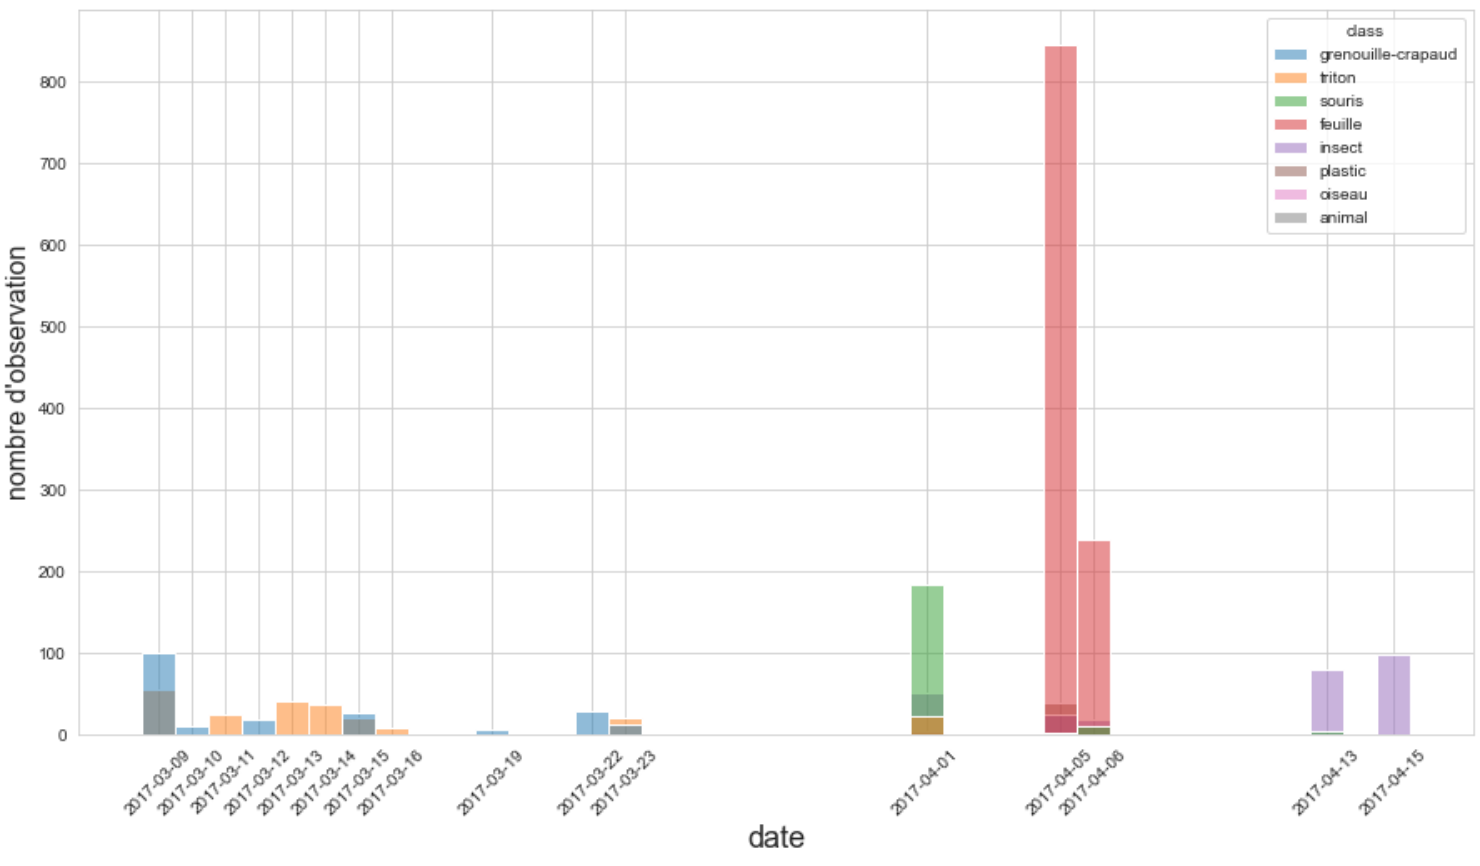
\includegraphics[width=300px]{images/filtre_observations_date.png}}
    \caption{Fréquentation des animaux en fonction de la date}
    \label{fig:Fréquentation des objets en fonction de la date}
\end{figure}

\begin{figure}[H]
    \centering
    \fbox{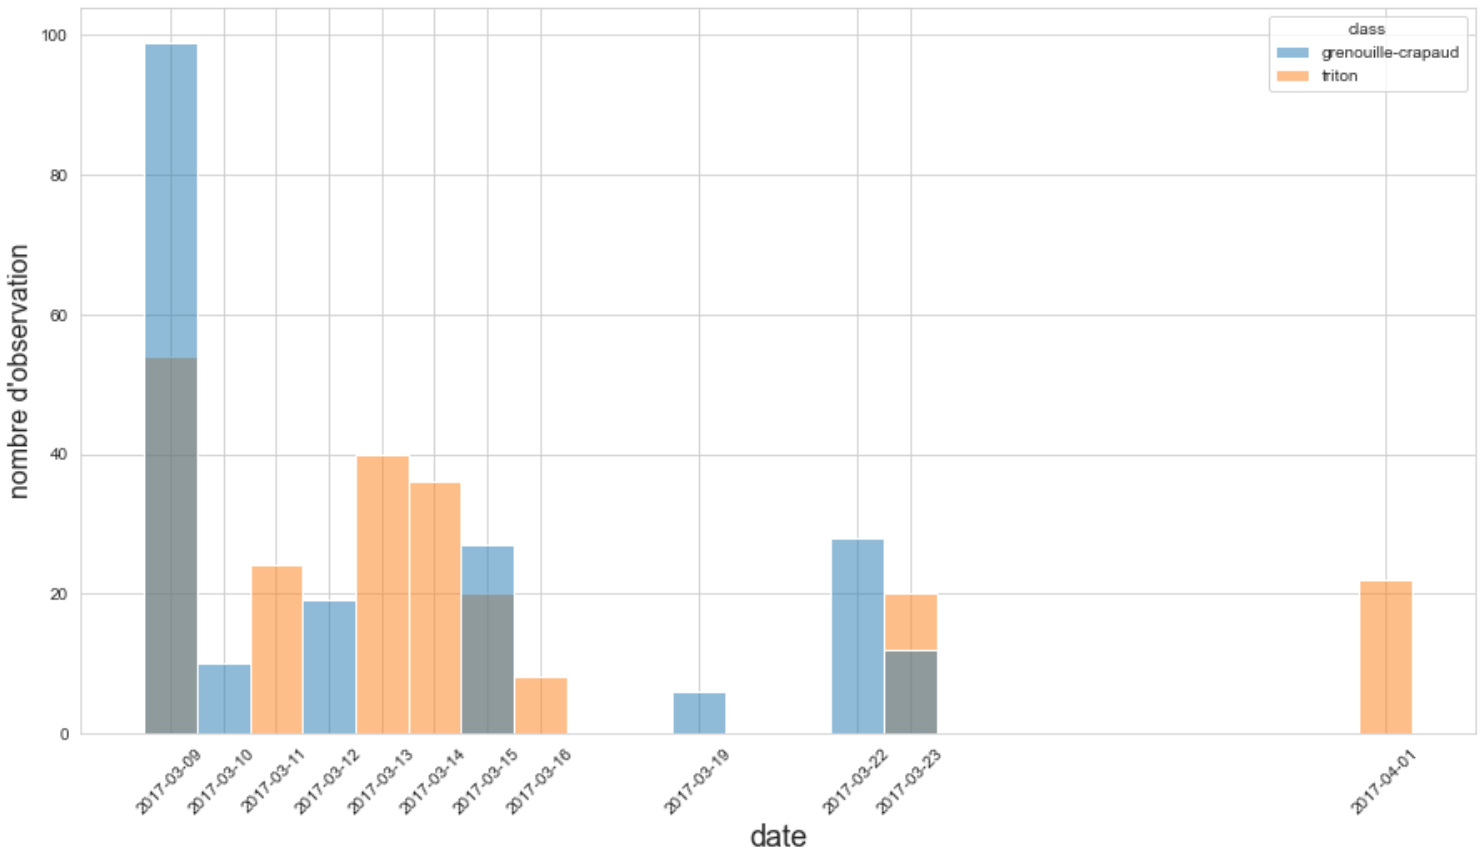
\includegraphics[width=300px]{images/filtre_crapGren_trit_date.png}}
    \caption{Fréquentation des batraciens observés en fonction de la date}
    \label{fig:Fréquentation des crapauducs en fonction de la date}
\end{figure}

\noindent On observe donc d'après la figure \ref{fig:Fréquentation des crapauducs en fonction de la date} que les batraciens d'intérêt utilisent particulièrement les crapauducs en mois de mars. Le reste des observations durant cette période, nous indique cependant que l'on observe peu de données en avril. \newline

Cependant, d'après cette ressource \footnote[1]{http://www.karch.ch/karch/home/amphibien/osservazione-di-anfibi.html} sur internet, les batraciens se reproduisent en fin février-début mars. On peut donc considérer que la déduction de fréquentation plus élevée des crapauducs par les batraciens en mars peut être considérée pour un premier filtrage pertinent des images.

\subsubsection{Heure}

\begin{figure}[H]
    \centering
    \fbox{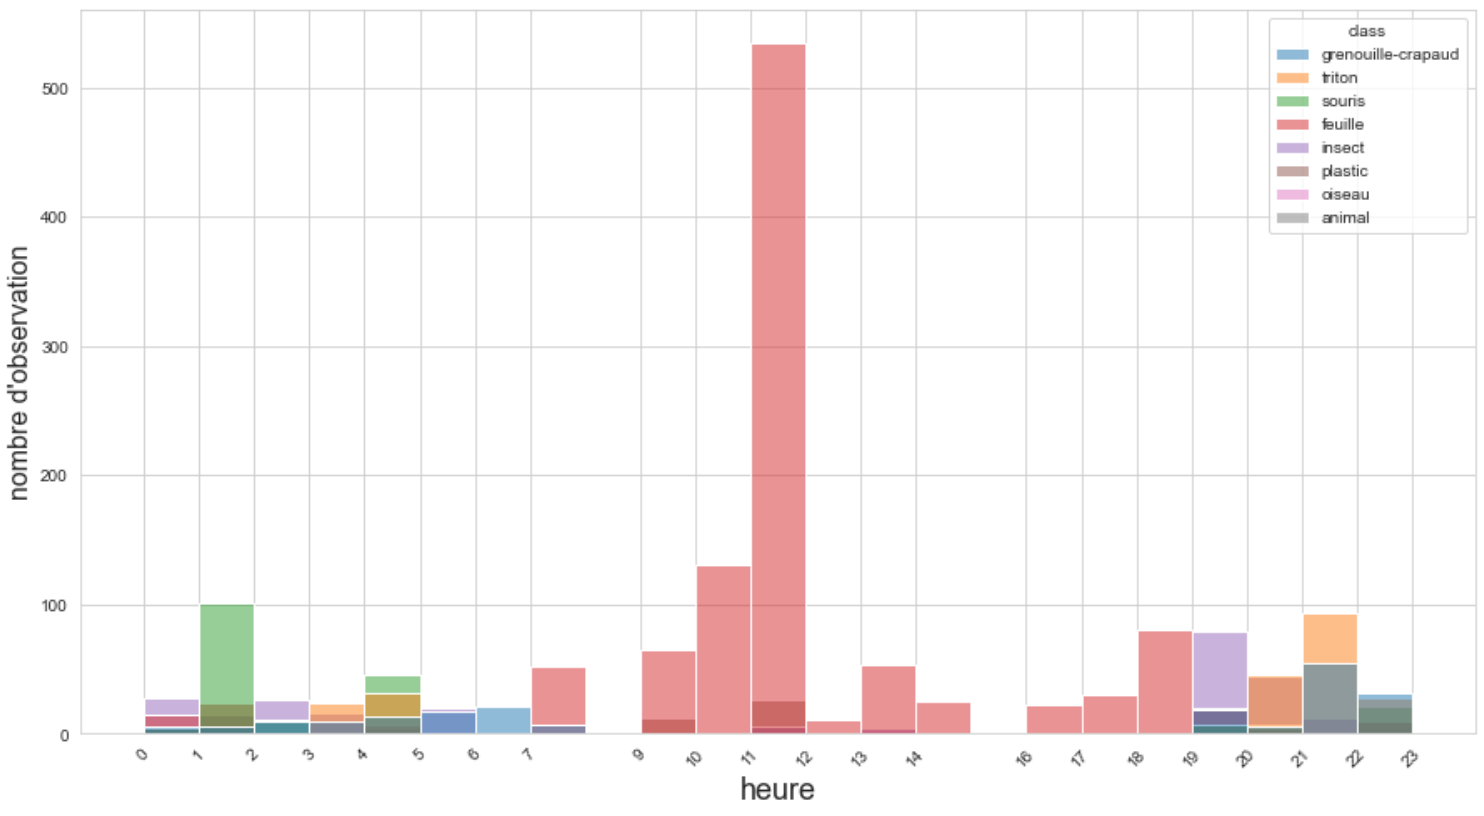
\includegraphics[width=300px]{images/filtre_observations_heure.png}}
    \caption{Fréquentation des animaux en fonction de l'heure}
    \label{fig:Fréquentation des objets en fonction de l'heure}
\end{figure}

On constate ici que le nombre de feuille étant plus grand que le reste d'objets observés, ceci nous empêche de pouvoir observer clairement la distribution d'observation d'objets. Visualisons donc les observations d'objets excepté les feuilles :

\begin{figure}[H]
    \centering
    \fbox{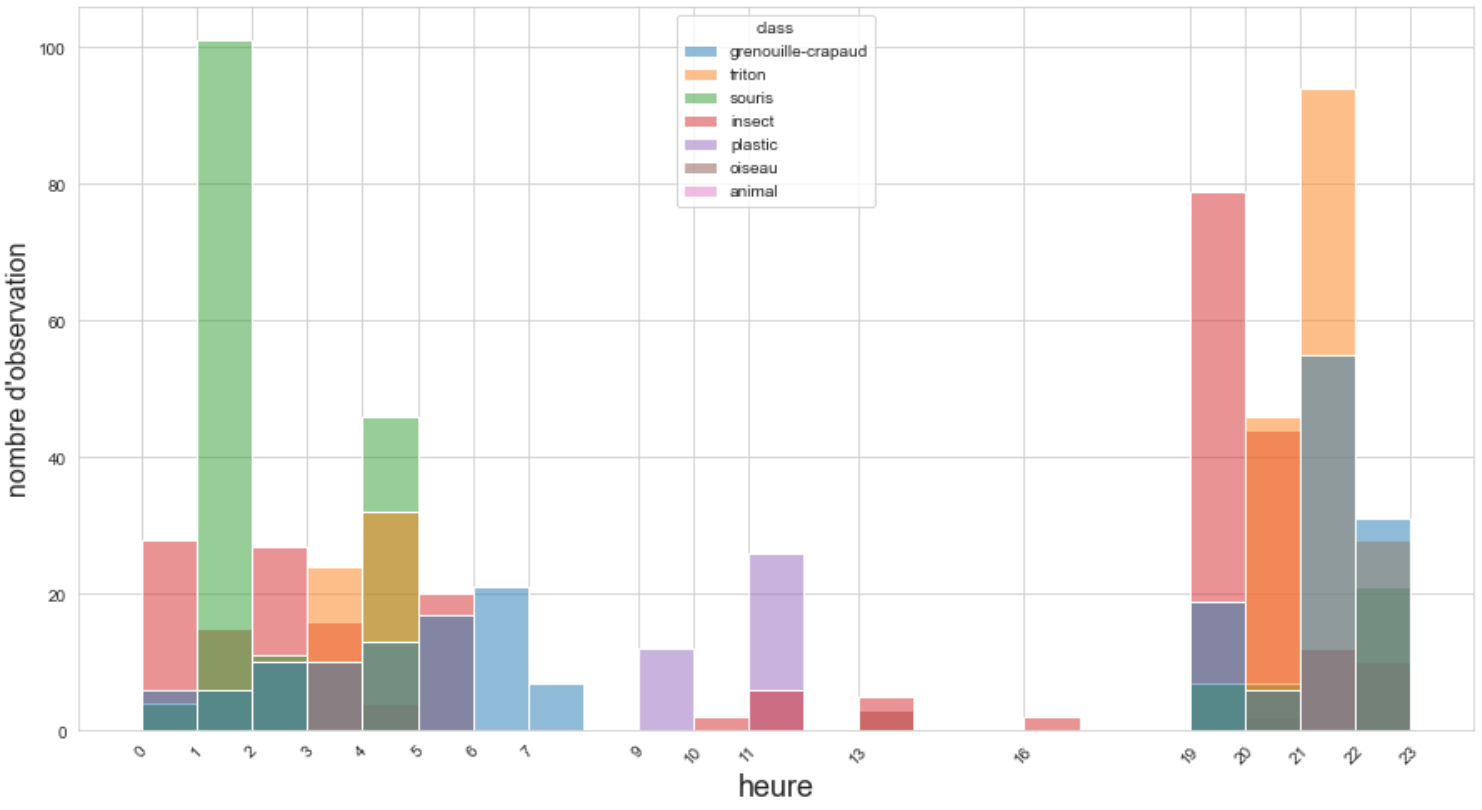
\includegraphics[width=300px]{images/filtre_observations_heure_sans_feuilles.png}}
    \caption{Fréquentation des batraciens observés en fonction de l'heure - sans les feuilles}
    \label{fig:Fréquentation des crapauducs en fonction de l'heure - sans les feuilles}
\end{figure}

\begin{figure}[H]
    \centering
    \fbox{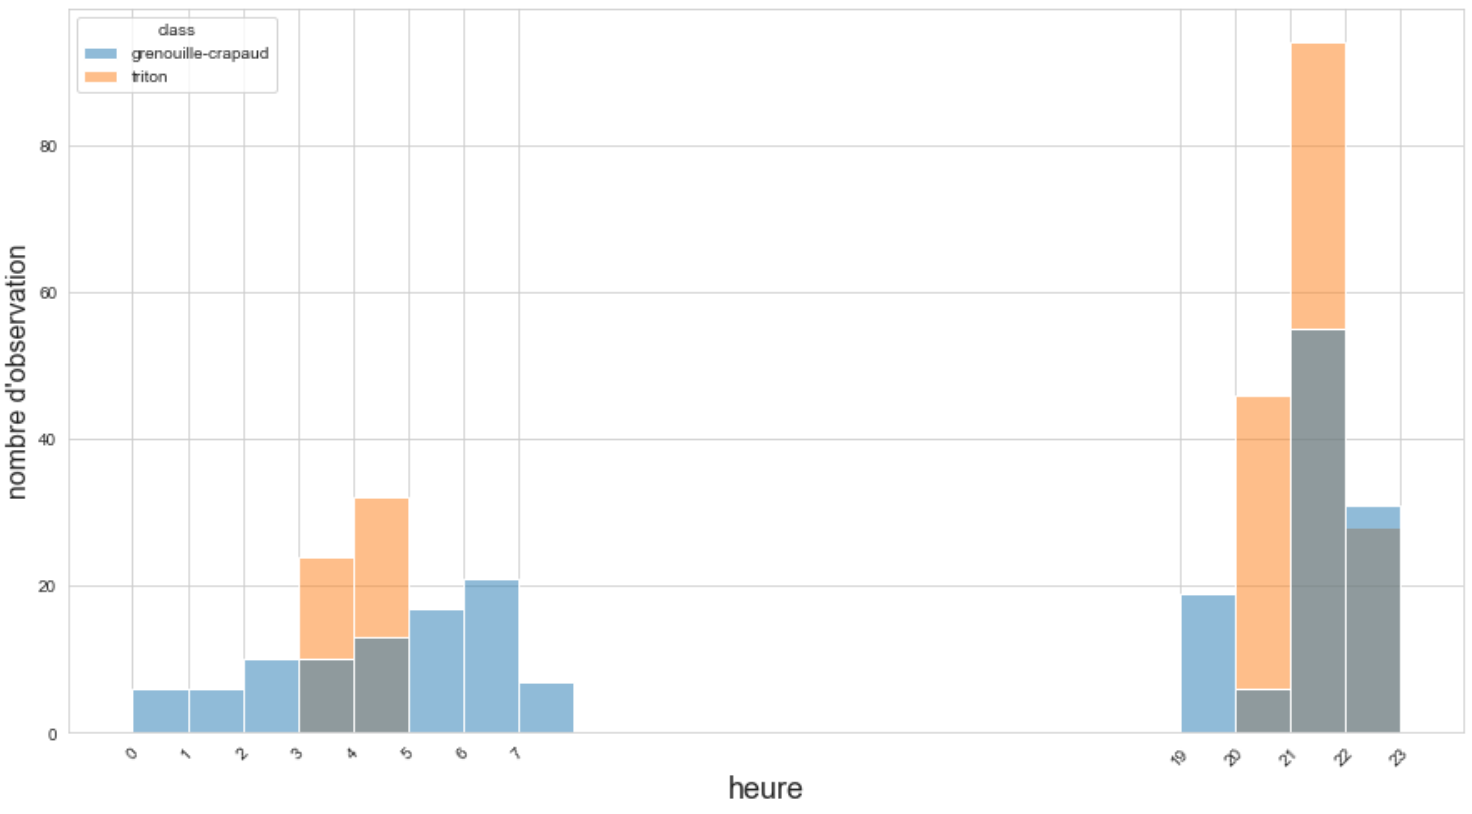
\includegraphics[width=300px]{images/filtre_crapGren_trit_heure.png}}
    \caption{Fréquentation des batraciens observés en fonction de l'heure}
    \label{fig:Fréquentation des crapauducs en fonction de l'heure}
\end{figure}

\noindent D'après la figure \ref{fig:Fréquentation des crapauducs en fonction de l'heure} ci-dessus, on observe que les batraciens d'intérêt utilisent particulièrement - même uniquement, pour cet ensemble de données - les crapauducs entre 19h et 7h du matin, c'est-à-dire de nuit. Le reste des observations (figure \ref{fig:Fréquentation des crapauducs en fonction de l'heure - sans les feuilles}) confirme premièrement la pertinence de cette observation, étant donné que nous avons une quantité élevée d'images prises tout au long de la journée parmi l'ensemble de données étudié ici.\newline

Les quelques recherches faites sur la période de déplacement des batraciens à l'étang indiquant également qu'elle est particulièrement durant le crépuscule, on confirme ainsi la pertinence que peut avoir ce deuxième filtrage des images.

% --

\subsection{Analyse météorologique}

Les données météorologiques additionnées des recherches en ligne ne sortent pas de particularité très prononcée quant à leur corrélation avec la fréquence d'observation de batraciens. Si l'on souhaite cependant citer les facteurs météorologiques qui pourraient être la plus déterministe, on citera l'humidité ; nous allons donc ici exposer nos observations la concernant. Notons que nous avons ici décidé de négliger les données labelisées "feuilles", comme elles forment du bruit et que nous avons fait un autre filtre s'en occupant si besoin.

\subsubsection{Humidité}

\begin{figure}[H]
    \centering
    \fbox{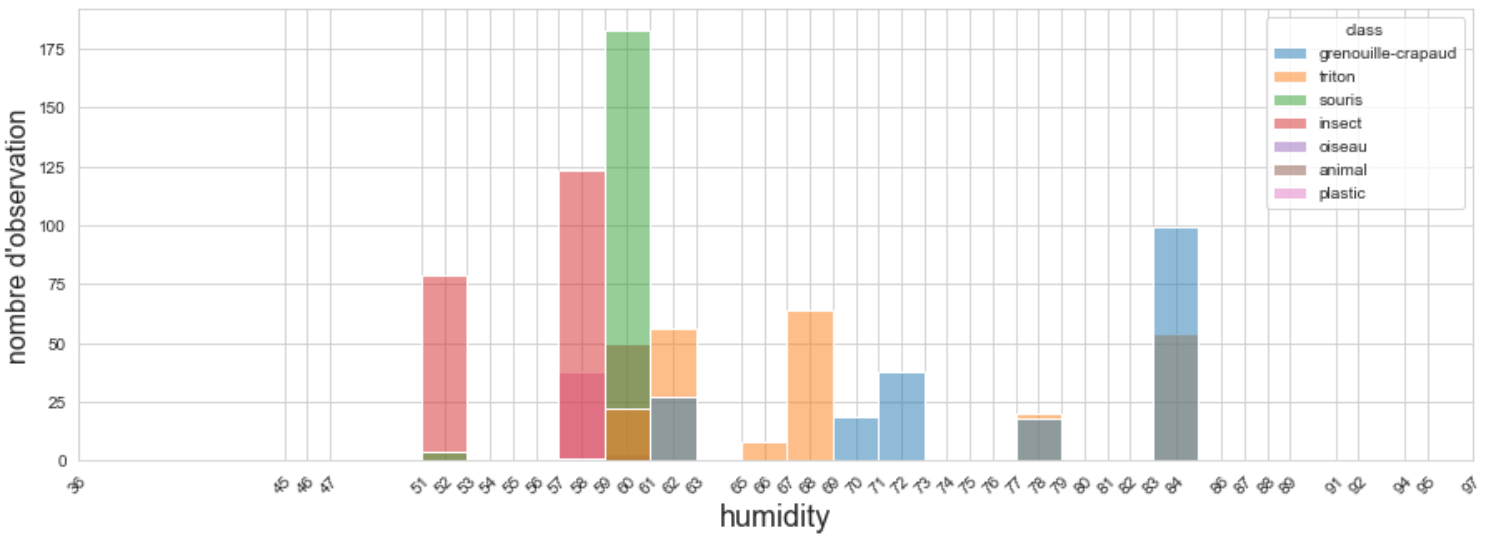
\includegraphics[width=300px]{images/filtre_meteo_observations_humidite.png}}
    \caption{Fréquentation des objets en fonction de l'humidité - sans les feuilles}
    \label{fig:Fréquentation des objets en fonction de l'humidité - sans les feuilles}
\end{figure}

\begin{figure}[H]
    \centering
    \fbox{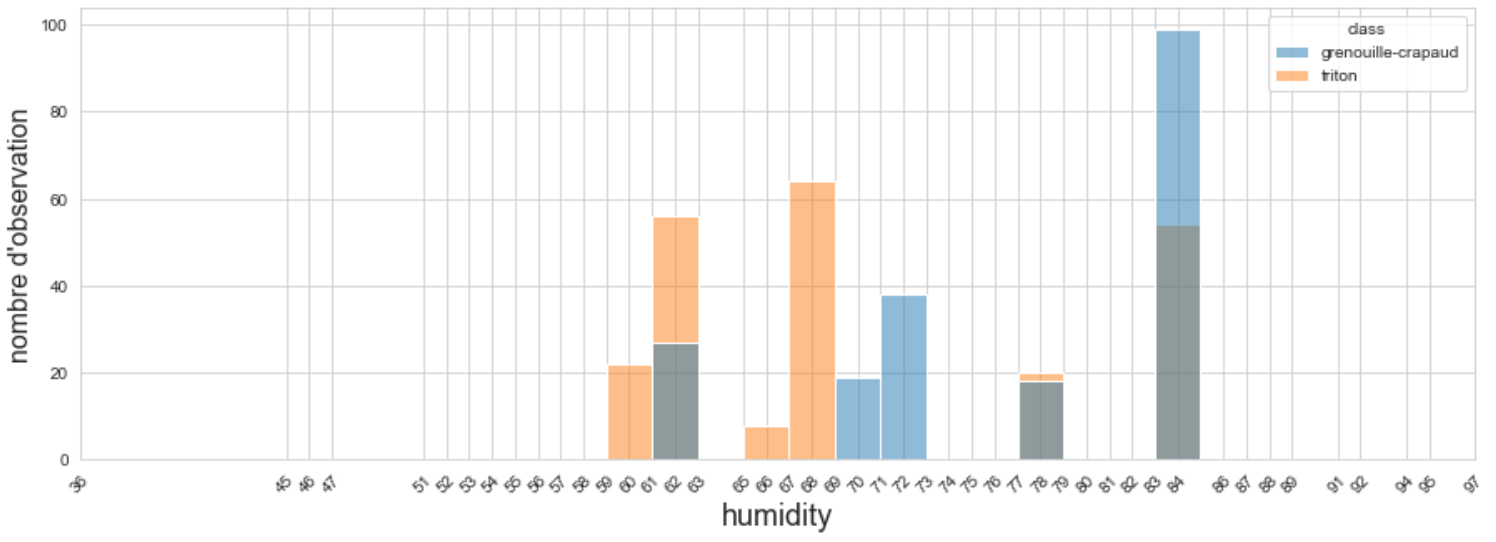
\includegraphics[width=300px]{images/filtre_meteo_crapGren_trit_humidite.png}}
    \caption{Fréquentation des batraciens en fonction de l'humidité - sans les feuilles}
    \label{fig:Fréquentation des batraciens en fonction de l'humidité - sans les feuilles}
\end{figure}

On voit ici qu'on peut imaginer prendre seulement les images prises lorsque l'humidité est au-dessus de 55.

% -------------------------------

\section{Détecteur de planches}\label{sex:Planche}

Nous avons développé un réseau de neurones convolutif à l'aide de la libraire PyTorch. Ce classificateur binaire prédit la présence ou non de planche.

\paragraph*{Dataset d'entraînement}

Nous avons extrait 600 images d'une même caméra et labellisé 359 non planches et 241 planches. Ensuite, nous avons développé un dataloader permettant d'intégrer nos labels et de charger des batchs de données directement dans la libraire PyTorch. Celui-ci, utilise un pipeline d'entrée qui applique plusieurs transformations à l'image avant de pouvoir l'utiliser comme un tenseur.

\begin{figure}[!htb]
    \centering
    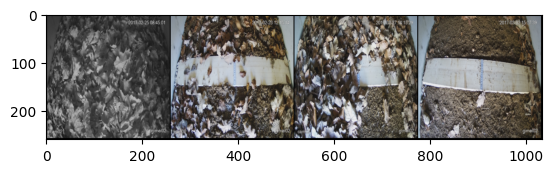
\includegraphics[width=200px]{images/filtre_exemple_data}
    \caption{Exemple de données d'entraînement}
    \label{fig:Entraînement du filtre}
\end{figure}

\paragraph*{Architecture du Détecteur}

Le détecteur est simplement constitué de 3 couches convolutives suivi de 2 couches entièrement connectées. Les channels d'entrée et de sortie des couches convolutives sont respectivement de : 3 - 32, 32 - 64, 64 - 128. Le nombre de neurones des couches fully connected sont de 128 et 1 pour le neurone de sortie. La fonction de coût utilisé est la BCELoss et l'optimiseur est Adam. Le réseau est entraîné pendant 10 epochs avec un learning rate de 0.001 et un momentum de 0.9 sur 3 epochs.

\begin{figure}[!htb]
    \centering
    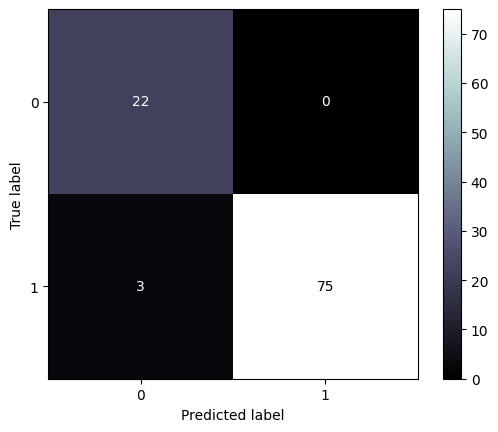
\includegraphics[width=200px]{images/filtre_cmatrix}
    \caption{Matrice de confusion du détecteur de planche}
    \label{fig:Matrice de confusion du filtre}
\end{figure}

\paragraph*{Résultats}


Nous avons calculé à partir de la figure \ref{fig:Matrice de confusion du filtre} que le détecteur de planche a une précision de 1 et un recall de 0.98 sur la détection de planche. En revanche, la précision sur la détection de non planche est de 0.88 et un recall de 1. Ces résultats signifient donc que notre filtre est un peu trop efficace et a tendance à se tromper pour détecter les images sans planche. Comme les résultats sont satisfaisant pour dégrossir le travail, nous n'avons pas passé de temps supplémentaire à optimiser le réseau afin qu'il sépare mieux les images dotés d'une planche ou non. Comme, nous traitons une grande quantité de données, l'erreur est acceptable. Lancé sur la quasi intégralité du dataset, le filtre a tourné pendant plus de 10h sur un ordinateur de bureau doté d'un processeur Ryzen9500X. Au final, le filtre a détecté 48910 images de non planches sur les 754543 images analysées. Il y a donc 10\% d'images de non planches qui ne seront pas exploitables. Via ce filtre, nous pourrions les écarter lors d'une future utilisation.


\chapter{Modèles}
\label{chap:Modeles}

\section{Choix des modèles}
Le choix des modèles a été un choix rapide.\newline
Nous avons commencé par regarder les tutoriels sur les sites web des frameworks que nous utilisons. Nous avons donc regardé les tutotiels de pytorch, car nous voulions utiliser ce framework en particulier, mais avons aussi regardé les githubs de modèles dont nous avions entendu parler, comme YOLOv5. Il faut noter que notre compréhension du problème et du jargon utilisé dans le domaine s’est enrichi au fur et à mesure de nos recherches. \newline 
Ainsi, nos premiers choix peuvent sembler mauvais, mais lors de la prise de décision nous étions persuadés de faire les bons choix. Notre approche de départ se basait essentiellement sur un facteur: nous voulions des modèles pour lesquels il existe beaucoup de ressources en ligne. Cette méthodologie nous a amené à explorer une solution (YOLOv5) qui n’était pas adaptée à notre problème. \newline
Après beaucoup d’essais infructueux, nous avons donc changé de méthodologie et nous nous sommes laissé la liberté d’utiliser des outils de plus haut niveau, tel que Detectron2 et de ne pas se restreindre uniquement à PyTorch. Une fois que nous avons pris en main ce framework, nous avons pu nous concentrer sur la performance du modèle. C'est aussi à ce stade que nous avons compris que le score sur le benchmark COCO2017 indiqué sur beaucoup de documentation de modèles était justement indiqué pour pouvoir comparer les modèles entre eux.

\section{Les échecs}
\subsubsection{YOLOv5}
YOLO est l'acronyme de You Only Look Once; il s'agit du premier modèle que nous avons essayé. Nous avons décidé de commencer avec ce modèle pour plusieurs raisons parmi lesquelles : une abondance de tutoriels sur le net et une solution qui nous semblait clé en main pour résoudre notre problème. Malgré ces signes positifs, il n’a pas été une solution adaptée. \newline
En effet, YOLO, a été publié il y a plusieurs année et n’est plus forcément l’état de l’art actuel. De plus, ce modèle est adapté à du traitement en temps réel ce qui ne fait pas partie de notre problème. Cependant, le réel souci qui nous a fait abandonner cette solution est la structure spéciale du dataset qui ne correspondait pas à notre structure. \newline 
Durant une phase de réflexion visant à résoudre le souci de structure, nous avons ainsi réalisé l’incapacité du modèle à gérer des images n’étant pas de 640x640 pixels. Nous aurions pu effectuer un réajustement de la taille des images mais ces derniers éléments nous ont fait réaliser que YOLO n’était pas la solution clé à laquelle nous nous attendions et avons décidé après quelques discussions de passer à un modèle plus adapté à notre problème initial. C'est ainsi que nous nous sommes lancé sur faster R-CNN, un modèle qui supporte des images de tailles arbitraires et qui est plus récent que YOLOv5.

\subsubsection{SSD}
\paragraph{} L'object detection étant une application nouvelle pour nous quand nous débutions le projet, après l'échec du modèle YOLO, nous avons décidé de nous lancer en parallèle sur différents modèles, le but étant de trouver celui ou ceux pouvant répondre efficacement à notre problématique. C'est dans cette optique que nous avons exploré le modèle SSD (Single Shot Multibox Détector). C'est un algorithme de detection d'objet dans une image qui au moment de la prédiction, divise l’image à l’aide d’une grille et génère des scores pour la présence de chaque catégorie d'objet dans chaque grille par défaut puis ajuste la grille pour mieux correspondre à la forme de l'objet. Le réseau combine ainsi les prédictions de plusieurs cartes de caractéristiques avec différentes résolutions pour traiter naturellement des objets de tailles diverses. Ce réseau se veut d'après la documentation, plus rapide que YOLO et aussi précis que FasterRCNN. 
\paragraph{} Nous avons trouvé un exemple d'implémentation sur \url{https://pytorch.org/hub/nvidia_deeplearningexamples_ssd}. La mise en oeuvre de celui ci s'est faite sans trop de douleur. Par la suite, il était question de faire du transfert learning ou fine tuning selon les documents. En effet, le modèle a été entrainé sur le dataset COCO (MS COCO: Microsoft Common Objects in Context) qui est un jeu de données d'images à grande échelle contenant 328 000 images d'objets quotidiens et d'êtres humains. Nous souhaitons donc ré-entrainer une partie du réseau avec notre set d'images. Pour ce faire nous nous sommes aidé d'un tutoriel trouvé sur git à l'adresse \url{https://github.com/Coldmooon/SSD-on-Custom-Dataset}. Dans celle ci est expliqué une façon d'entrainer le modèle SSD sur un dataset personnalisé avec pour contrainte que les images doivent être de taille 300*300 ou 512*512. Travailler sur des images carrées était l'un des problèmes que nous avons rencontré avec YOLO, mais nous avons pensé résoudre ce problème avec les fonctions de resizing existantes. 
Nous avons ccommencé par éssayer de reproduire le tuto sur le dataset proposé dans celui-ci. A de nombreuses reprises, nous avons fait face à des erreurs dont nous ignorions la provenance ainsi que la solution. Pour finir cela nous a pris beaucoup de temps pour au final ne pas arriver à entrainer le modèle sur le dataset en question. Nous n'avons donc pas pu aller au bout de cette implémentation. Mais nous restons convaincus que ça reste une alternative à la résolution de notre problématique.

\subsubsection{Faster R-CNN avec Keras}

\paragraph{} Après l'échec de YOLOv5 en raison de la nécessité d'utiliser des images carrées de taille fixe, nous avons décidé de nous pencher sur une utilisation potentielle d'un réseau de neurones de type Faster R-CNN, plus précisément en utilisant la bibliothèque open-source Keras puisque c'est une bibliothèque que nous avions déjà utilisée auparavant dans le cadre du cours sur les réseaux de neurones. Pour atteindre cet objectif, nous avions à disposition une implémentation toute faite de Faster R-CNN utilisant Keras disponible à l'adresse suivante : \url{github.com/you359/Keras-FasterRCNN}. Malheureusement, nous avons rencontré un certain nombre de problèmes au moment d'utiliser l'implémentation fournie.

\paragraph{} Tout d'abord, il s'agit d'un code plutôt ancien qui n'est pas forcément compatible avec les dernières versions des librairies utilisées en Python. En effet, ces librairies sont régulièrement mises à jour et certaines fonctions disponibles sont alors dépréciées, modifiées voire même définitivement supprimées. Il a donc fallu trouver par tâtonnement les bonnes versions des librairies à utiliser en créant de multiples environnements virtuels à l'aide de conda et en intérprétant les divers messages d'erreur énigmatiques renvoyés à chaque nouvelle tentative. Finalement, nous avons réalisé que le repo github contenait un fichier texte indiquant les versions optimales des librairies à utiliser pour ce projet. Cependant, même en utilisant les versions recommandées, le code continuait à planter après quelques secondes pour d'obscures raisons.

\paragraph{} Ensuite, le second problème réside dans la documentation de l'implémentation de Faster R-CNN qui contient ce qui semble être une grossière erreur quant à la version de Python à utiliser. En effet, nous avons appris au point précédent qu'il valait mieux lire attentivement la documentation disponible avant de se lancer corps et âme dans le code. Or cette documentation indique explicitement d'utiliser Python 2 pour faire tourner le code mis à disposition. Malheureusement, même en utilisant les bonnes versions des librairies et de python le code ne voulait définitivement pas fonctionner. Dans une tentative désespérée nous avons donc changé la version de Python pour Python 3 et là, comme par magie, le code commence à tourner et le réseau de neurones commence à s'entraîner.

\paragraph{} Finalement, nous arrivons au problème principal que nous n'avons jamais réussi à résoudre et qui est donc la raison pour laquelle nous avons abandonné ce modèle. En effet, même si le code parvenait désormais à se lancer correctement, il plantait maintenant à des étapes aléatoires de l'entraînement du réseau de neurones, parfois après quelques secondes, parfois après quelques dizaines de minutes, mais toujours en renvoyant une grande quantité de messages d'erreur pratiquement incompréhensibles. Malgré de longues et intenses recherches sur de mutliples sites internet et forums, personne ne semblait en mesure de trouver une solution à ce problème. En effet, d'autres utilisateurs rencontraient le même souci mais la solution adoptée au final était toujours la même : changer de modèle, souvent pour passer sur detectron qui possède une documentation beaucoup plus complète, ce que nous avons donc également fait par la suite. Nous avons tout de même réussi à finir un entraînement sans encombre, mais pour y parvenir il a fallu réduire drastiquement le nombre d'epochs afin de limiter la durée de l'entraînement, et à la fin de celui-ci le réseau de neurones n'était pas capable de reconnaître quoi que ce soit sur les images, probablement en raison du manque d'entraînement.

\paragraph{} Pour conclure, on peut donc dire que le coeur du problème de l'implémentation utilisée est son manque de popularité dans la communauté du data science. En effet, comme les utilisateurs sont peu nombreux, des erreurs se glissent dans la documentation et passent inaperçues tandis que d'autres problèmes restent à jamais non-résolus car personne ne semble connaître la solution. Nous avons donc choisi d'utiliser par la suite des modèles plus populaires et par conséquent mieux documentés. 

\section{Les réussites}

\subsection{Detectron2}
Detectron2 est une puissante plateforme de détection d'objets et de segmentation d'images développée par Facebook AI Research (FAIR). Il s'agit de la deuxième génération du système Detectron original, également développé par FAIR. Detectron2 est conçu pour être hautement modulaire et flexible, et il est utilisé pour un large éventail de tâches de computer vision, comme la détection d'objets, la segmentation d'instances, la segmentation panoptique, et plus encore. Il est construit au-dessus du framework PyTorch et présente une variété de modèles de pointe. L'utiliser nous a permis de facilement changer de modèle une fois que notre code d'entrainement était fonctionnel.
En effet, beaucoup de configuration se font à travers le fichier de configuration, c'est dans lui qu'on spécifie les détails du processus d'entrainements tels que le set de données d'entrainement, le set de validation, le modèle à entrainer, le learning-rate etc. De plus, il intégre de nombreuses configuration de bases et grâce à ceci nous n'avons qu'à changer les paramètres qui nous intéressent comme : la backbone du modèle, les poids à charger pour faire du transfert learning. Detectron2 intégre directement dans la class \verb|DefaultTrainer| une méthode qui affiche des statistiques sur l'entrainement en cours, comme le nombre d'epochs, le learning-rate, le temps restant, etc. Cela nous a permis de suivre l'entrainement de nos modèles. Il s'occupe aussi de faire de l'augmentation de données durant le processus d'entrainement. Finalement, Detectron2 fournit aussi pour tous ses modèles des poids après entrainement du modèle.
\paragraph{}
Entrainer un modèle avec Detectron2 se résume donc à faire un code similaire à celui visible en ci-dessous.
\lstset{language=Python}
\begin{lstlisting}
from detectron2 import model_zoo
from detectron2.engine import DefaultPredictor
from detectron2.config import get_cfg
cfg = get_cfg()
# On charge une configuration de base
cf_file="COCO-Detection/faster_rcnn_X_101_32x8d_FPN_3x.yaml"
cfg.merge_from_file(model_zoo.get_config_file(cf_file))
cfg.DATASETS.TRAIN = ("triton_train",)
cfg.MODEL.WEIGHTS = model_zoo.get_checkpoint_url(cf_file)  
# cfg.params... voir dans la documentation
trainer = DefaultTrainer(cfg) 
trainer.resume_or_load(resume=False)
trainer.train()
predictor = DefaultPredictor(cfg)
\end{lstlisting}
\paragraph{}
En conclusion Detectron2, nous avons a permis de facilement changer de modèle et de tester plusieurs modèles. Nous avons aussi pu facilement faire du transfert learning en chargeant les poids d'un modèle pré-entrainé. 


\subsection{FASTER R-CNN}

Le modèle d'apprentissage automatique Faster R-CNN (R-CNN pour "Region-based Convolutional Network") vient à la base du modèle R-CNN, qui a été ensuite amélioré pour former le modèle Fast R-CNN, qui a lui-même finalement été optimisé pour créer le modèle Faster R-CNN étudié ici. R-CNN, Fast R-CNN et Faster R-CNN sont tous des modèles de traitement de l'image utilisés pour la détection d'objets dans les images. Ils utilisent tous une approche en plusieurs étapes qui consiste à extraire des caractéristiques de l'image à l'aide d'un réseau de neurones convolutionnel (CNN), puis à identifier les régions de l'image qui pourraient contenir des objets à l'aide de la sélection de région d'intérêt (ROI) et enfin à prédire la classe de chaque région sélectionnée et à localiser l'objet dans l'image.

\paragraph{R-CNN} est un modèle datant de 2014, dont on peut voir l'article scientifique \href{https://arxiv.org/pdf/1311.2524.pdf}{\textit{ici}}. Voici premièrement son architecture en figure \ref{fig:rcnn_architecture} ci-dessous.

\begin{figure}[H]
    \centering
    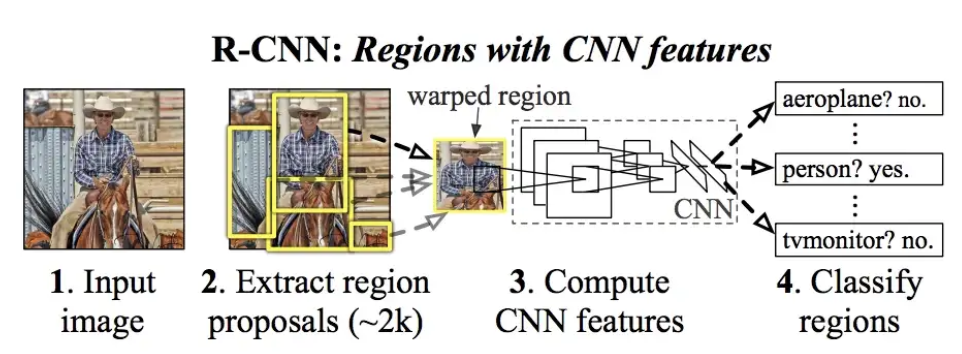
\includegraphics[width=300px]{images/model_rcnn_architecture.png}
    \caption{Architecture de R-CNN}
    \label{fig:rcnn_architecture}
\end{figure}

Comme dit précédemment, il s'agit du modèle original. Il est très performant, mais aussi très lent, car il traite chaque région sélectionnée de manière indépendante et entraîne un modèle de classification séparé pour chaque région.

% ---

\paragraph{Fast R-CNN} date d'une année plus tard, soit de 2015. On trouve son article scientifique \href{https://arxiv.org/pdf/1504.08083.pdf}{\textit{ici}} et voici son architecture en figure \ref{fig:fastRcnn_architecture} ci-dessous.

\begin{figure}[H]
    \centering
    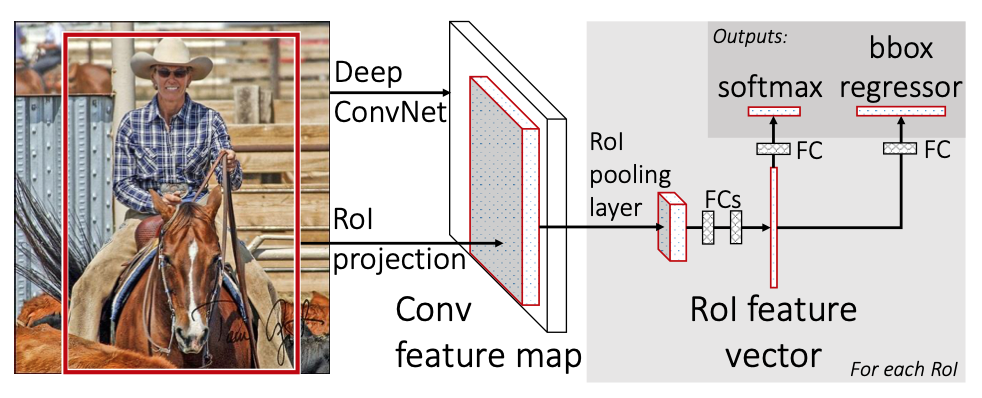
\includegraphics[width=250px]{images/model_fastRcnn_architecture.png}
    \caption{Architecture de Fast R-CNN}
    \label{fig:fastRcnn_architecture}
\end{figure}

Fast R-CNN est ainsi une version améliorée de R-CNN, qui est beaucoup plus rapide. Au lieu de traiter chaque région sélectionnée de manière indépendante, Fast R-CNN utilise un seul modèle de classification pour toutes les régions sélectionnées dans l'image. De plus, il utilise une technique appelée "max pooling régional" pour réduire la dimension des régions sélectionnées avant de les passer au modèle de classification.

% ---

\paragraph{Faster R-CNN} vient une année plus tard encore, en 2016.  \href{https://arxiv.org/pdf/1506.01497.pdf}{\textit{Ici}} se trouve son article scientifique, et voici finalement son architecture ci-dessous, en figure \ref{fig:fasterRcnn_architecture}.

\begin{figure}[H]
    \centering
    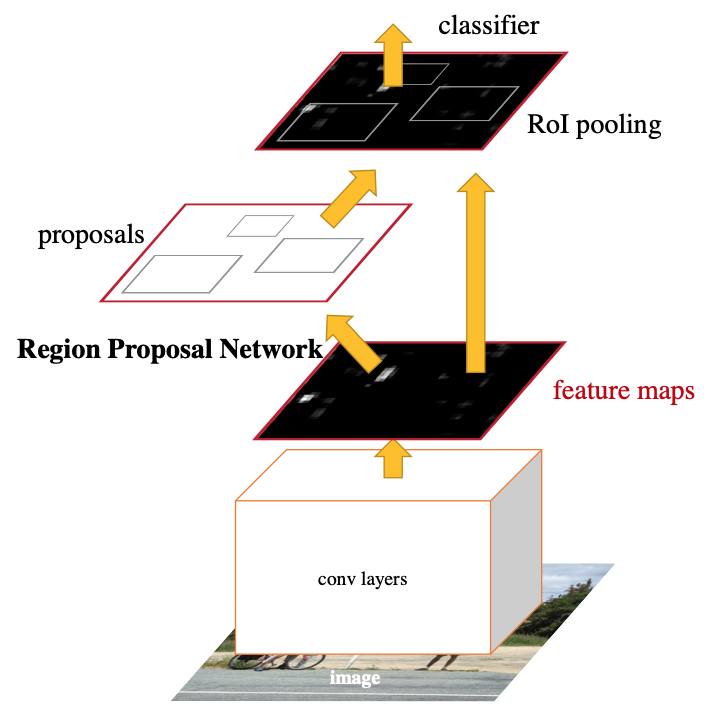
\includegraphics[width=250px]{images/model_fasterRcnn_architecture.png}
    \caption{Architecture de Faster R-CNN}
    \label{fig:fasterRcnn_architecture}
\end{figure}

\paragraph{} Faster R-CNN est effectivement un modèle encore plus rapide que Fast R-CNN. Il utilise une technique appelée "réseau de proposition de région" (RPN) pour identifier automatiquement les régions de l'image qui pourraient contenir des objets, sans avoir besoin de calculer explicitement toutes les régions de l'image comme le font R-CNN et Fast R-CNN. Cela permet à Faster R-CNN de traiter l'image de manière beaucoup plus rapide et de détecter des objets avec une précision comparable à celle de Fast R-CNN.

\paragraph{} Nous avons décidé d'utiliser une backbone \verb|X_101_32x8d_FPN| c'est à dire un réseau ResNeXt-101 avec une configuration de 32 groupes de large de 8, 32x8d fait donc référence à des hyper-paramètres utilisé par le réseau ResNeXt de la backbone. Nous n'avons pas nous même cherché ces valeurs, nous avons choisis cette configuration en copiant la configuration de Faster-RCNN donnant le meilleur score COCO selon la documentation de Detectron2. Ce réseau ResNeXt est suivit d'un second réseau, FPN cette fois, qui forment ensemble l'entièreté de la backbone que nous utilisons.

\paragraph{} Pour des raisons évidentes de rapidité de traitement des images, nous avons donc investigué plus précisément ce dernier modèle - Faster R-CNN - pour notre problème. C'est d'ailleurs ce modèle que nous avons finalement sélectionné pour répondre à la problématique de ce projet, comme mentionné ci-après, en chapitre \autoref{chap:Evaluation} de ce rapport ("Evaluation").\newline
Pour se faire, nous avons donc du adapter les exemples trouvés sur internet à notre problème, légèrement différent de ces dits exemples. Il a donc fallu assembler différents tutoriels, ce qui a impliqué beaucoup de temps d'analyse et de compréhension. Aussi, nous avons du nous habituer au jargon technique que nous n'avions pas - tel que mAP et les benchmarks coco pour en citer quelques uns. Il a également fallu passer du temps pour comprendre ce qu'était COCO (Common Object in COntext) : une base de données fournie par Microsoft qui contient des images annotées avec des informations sur les objets présents dans chaque imag et qui fourni également un benchmark ; un ensemble de tests et de métriques utilisés pour évaluer les performances des modèles de reconnaissance d'objets et de segmentation d'images.

% ------------------------------------------

\subsection{RETINA net}

\paragraph{Description}

\paragraph{} RetinaNet est un réseau de neurones convolutionnel utilisé en détection d'objets dans des images. Il a été présenté dans le papier "Focal Loss for Dense Object Detection" de Tsung-Yi Lin et al. en 2017.

\paragraph{} Le principe de base de RetinaNet est de prédire des scores de confiance pour chaque classe d'objet à chaque position de l'image, ainsi qu'une boîte englobante pour chaque objet détecté. Pour cela, RetinaNet utilise une architecture de réseau de neurones à deux branches, l'une pour prédire les scores de confiance et l'autre pour prédire les boîtes englobantes.

\paragraph{} La particularité de RetinaNet est qu'il utilise une "perte focale" pour lutter contre l'asymétrie des données dans les jeux de données de détection d'objets. Dans ces jeux de données, il y a souvent beaucoup plus de fond (c'est-à-dire des parties de l'image qui ne contiennent pas d'objets) que d'objets détectables. Cette asymétrie peut rendre difficile l'apprentissage pour le modèle, car il y a moins d'exemples d'objets à apprendre. La perte focale atténue cet effet en diminuant la contribution des exemples faciles (c'est-à-dire ceux où l'objet est facilement identifiable) à la perte totale, ce qui permet au modèle de se concentrer davantage sur les exemples difficiles.

\paragraph{} Le modèle RetinaNet est souvent utilisé dans les tâches de détection d'objets pour améliorer la précision et réduire le nombre de faux positifs. Il a été largement utilisé dans de nombreuses applications, notamment la reconnaissance de la circulation routière et la reconnaissance de la faune.

\paragraph{} Nous avons décidé d'utiliser une backbone \verb|R_101_FPN| c'est à dire un réseau ResNet-101 suivit d'un réseau FPN. Il s'agit selon la documentation de Detectron2 de la backbone qui donne un modèle RetinaNet le plus précis, c'est à dire donnant le meilleur score sur le benchmark COCO. Nous avons donc choisi ce modèle pour avoir un modèle précis et qui puisse être utilisé pour répondre à notre problématique de base.

\paragraph{} En résumé, RetinaNet est un modèle de détection d'objets qui utilise une architecture à deux branches et une perte focale pour améliorer la performance de détection dans les jeux de données asymétriques.

\paragraph{Results}

\paragraph{} Ce modèle obtient des résultats extrêmement satisfaisants. En effet, il s'agit du modèle qui détecte les crapauds/grenouilles avec la plus grande accuracy. Les résultats précis de ce modèle sont par ailleurs détaillés dans la section "Evaluation" du \autoref{chap:Evaluation} de ce rapport.

\subsection{\textit{De}tection \textit{Tr}ansformer (\textit{DE-TR)}}

\href{https://github.com/facebookresearch/detr}{DETR} est un modèle sorti en 2020 qui est extrêmement simple à implémenter et fournit des scores (mAP, IoU etc) sur le benchmark COCO qui surpassent ceux des modèles existants de quelques points. C’est pourquoi, en plus de son architecture innovante, nous avons voulu l’essayer. L’architecture, visible en figure \ref{fig:detr_architecture}, se base sur un transformer, un modèle de deep learning parut dans le fameux papier de 2017 de Google, \href{https://arxiv.org/pdf/1706.03762.pdf}{\textit{Attention is all you need}}. On peut observer que le modèle commence par générer des features à partir de l'image d'entrée en utilisant une backbone, c'est-à-dire un modèle pré-entrainé visant justement à extraire ces features à l'aide d'un réseau neuronal convolutif. Ensuite, le modèle utilise la partie encodeuse du transformer suivi de son équivalent décodeur et finalement d'un "prediction feed-forward networks" (FFN). C'est le réseau FFN qui génère les possibles bounding boxes et les classes associées.

\begin{figure}[th!]
    \centering
    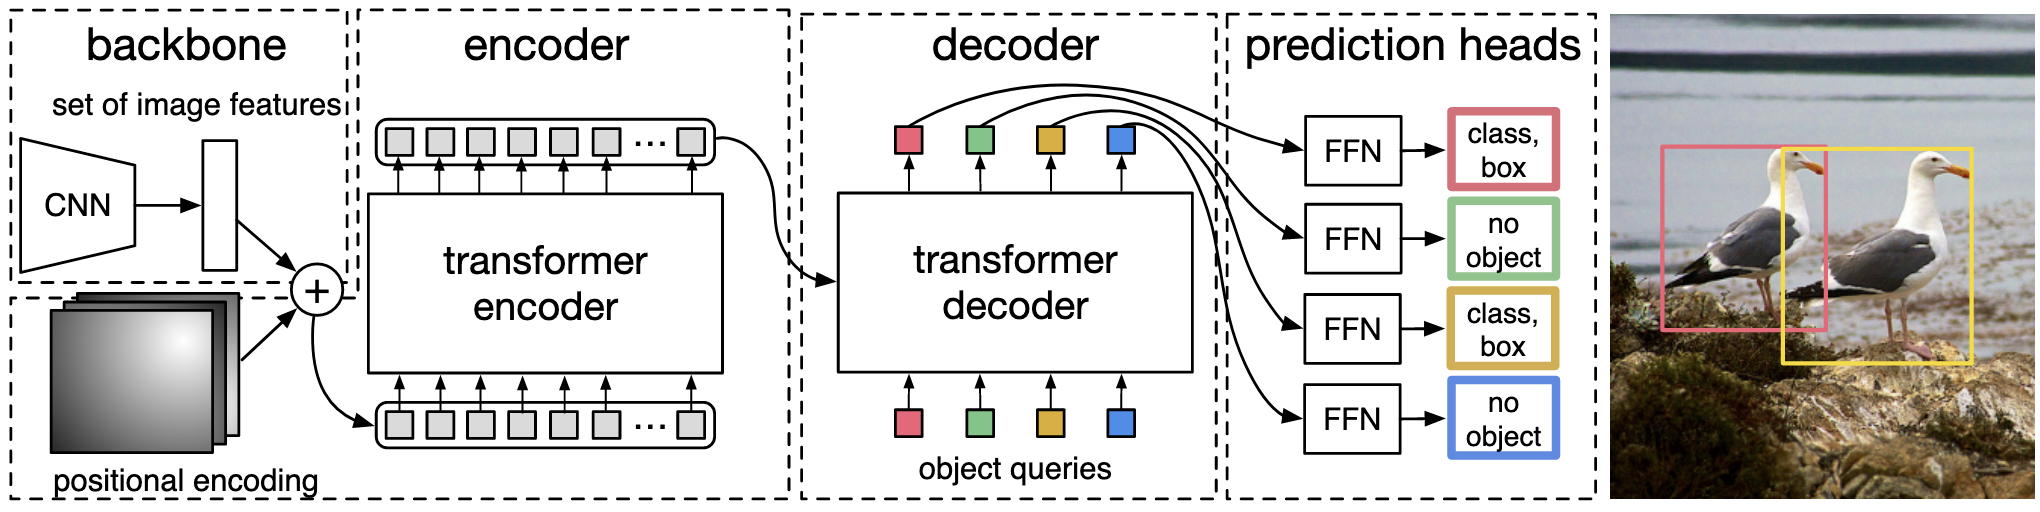
\includegraphics[width=\textwidth]{images/detr_architecture.png}
    \caption{Architecture de DETR}
    \label{fig:detr_architecture}
\end{figure}
% ----------------------------------------------------
Ce modèle est simple car il utilise peu de couches contrairement à FasterRCNN par exemple. Une implémentation PyTorch est faisable en 60 lignes. Cependant, l'entrainement est complexe et nous nous y sommes repris plusieurs fois pour réussir un entrainement.
DETR n'est pas un modèle fournit dans les configurations de bases de Detectron2. Sur le dépôt github du projet DETR, du code permettant de l'intégrer avec Detectron2 est fournis, néanmoins ce wrapper est complexe à utiliser et nous n'avons pas réussis à obtenir des résultats satisfaisants, notre hypothèse est qu'il n'y as pas de threshold sur les probabilités de classes. Ainsi nous avons des prédictions similaires à celle visible sur la figure \ref{fig:detr_predictions_threshold} qui illustre le problème.
\begin{figure}[h!]
    \centering
    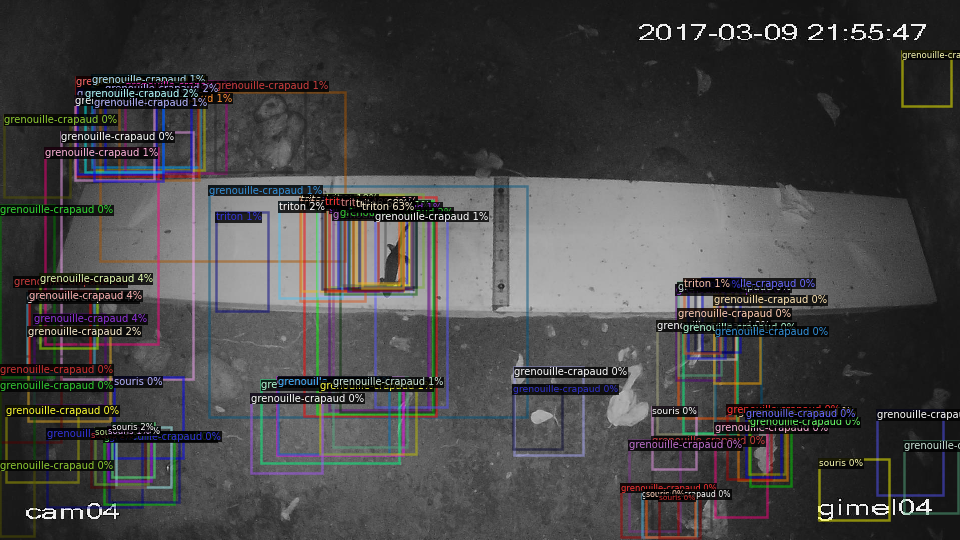
\includegraphics[width=\textwidth]{images/detr_threshold.png}
    \caption{Prédiction de DETR après un entrainement sur un GPU premium}
    \label{fig:detr_predictions_threshold}
\end{figure}

Nous pouvons observer que le triton au centre de l'image est correctement reconnu avec une probabilité de 63\% mais qu'il y a trop de bounding boxes. Nous voulions implémenter un système de filtrage après le modèle. Cependant nous n'avons pas réussis car le modèle ayant beaucoup de poids, il nécessitait un GPU puissant pour être entrainé. Nous avons déjà dépensé beaucoup d'argent de notre poche sur le service google colaboratory et nous n'avions pas les moyens de payer à nouveau pour entrainer et experimenter sur un GPU puissant. Nous avons donc abandonné l'idée de filtrer les bounding box. Vous pouvez néanmoins retrouver notre implémentation de DETR ici \url{https://colab.research.google.com/drive/1nJC4tI83L1_sLhfFUMZPk4bFN0Ui3Jfi?usp=sharing}. Une version ayant tourné une fois sur un GPU premium est disponible sur github sous le même nom.

Nous avons tenté une seconde implémentation de DETR en codant en PyTorch le modèle puisque on peut le faire en 60 lignes. L'entrainement était optimisé avec PyTorch Lightning. Nous avons réussis l'entrainement cependant en n'utilisant pas Detectron2, nous n'avons cette fois pas réussis à obtenir des scores sur le benchmark COCO fournit dans la class \verb|COCO_Evaluator| de Detectron2. Nous avons testé sur quelques images et voyons des bons résultats, de plus durant l'entrainement de bonnes métriques sont affichées cependant sans benchmark COCO, il est difficile de comparer ce modèle aux autres. Vous pouvez retrouver notre implémentation ici: \url{https://github.com/student-GML/crapauduc/blob/main/model_finaux/DETR_kaggle_fine_tune.ipynb}

En résumé : Nous n'avons pas réussis par manque de ressources à filtrer les probabilités faibles avec le wrapper Detectron2 de DETR. Nous avons cependant, avec PyTorch Lightning, réussis à avoir de bons scores durant l'entrainement. Ces résultats ne sont pas suffisants pour être comparés aux autres modèles. Et nous avons donc décider d'en rester là avec ce modèle.

\section{Modèles évalués}
D'après ces nombreuses recherches, nous avons donc implémenté et évaluer deux modèles fonctionnels dont nous avons pu comparer les scores d'évaluation sur des données tests : 

\begin{itemize}
    \item[-] Faster R-CNN avec Detectron2 ;
    \item[-] Retinanet avec Detectron2.
\end{itemize}
\chapter{Analyses}
\label{chap:Evaluation}
Nous allons commencer par expliquer les différentes métriques utilisables lors d'une tâche d'object detection. Ensuite, nous allons expliquer comment lire un benchmark COCO. Enfin nous allons analyser l'entrainement de nos différents modèles ainsi que le score COCO obtenu. Et pour finir, nous allons observer et analyser des images qui présentent des erreurs de prédictions.

\section{Contexte}
Dans une tâche d'object detection, nous utilisons le score IoU qui signifie Intersection over Union.
C'est un score qui compare les bounding boxes prédites par le modèle avec les bounding boxes réelles (ground-truth).
Une tâche d'object detection comprend deux sous-problèmes: la classification et la localisation.
Ainsi nous avons plusieurs métriques pour analyser la performance d'un modèle. IoU se concentre sur 
la localisation des bounding boxes prédites tandis que la métrique mAP (mean Average Precision) 
se concentre sur la classification.
\begin{figure}[bh!]
    \centering
    \scalebox{0.5}[0.5]{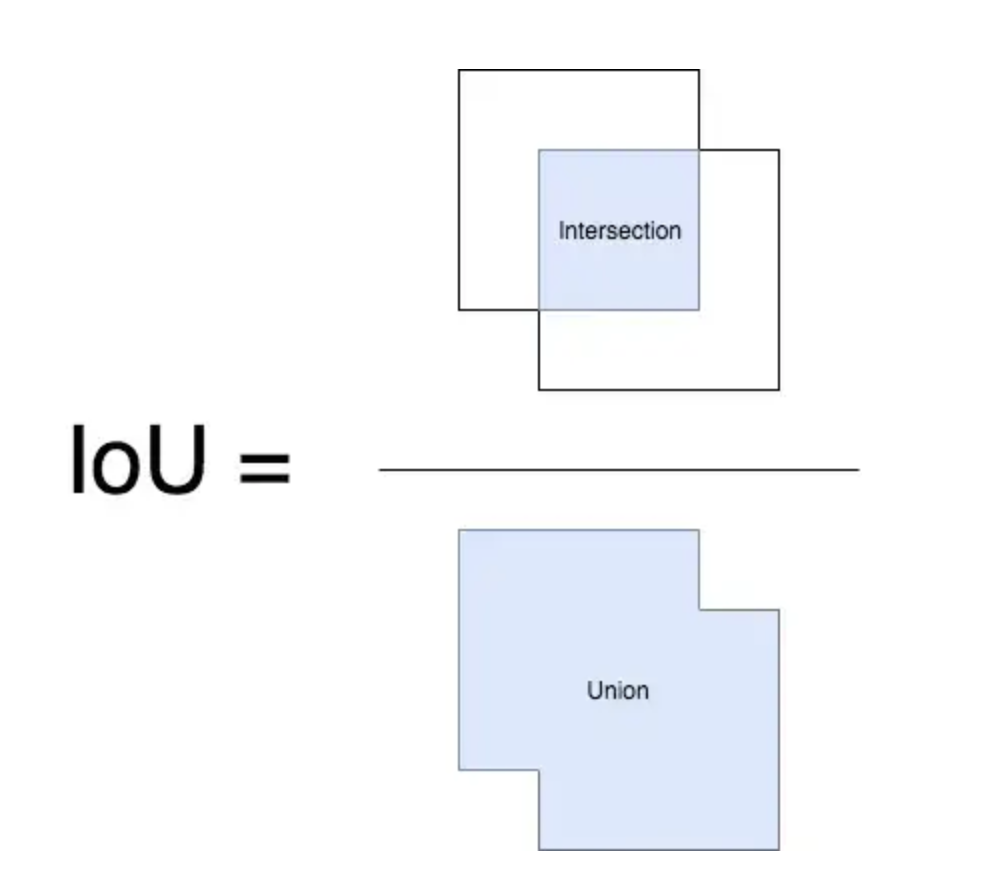
\includegraphics[width=\textwidth]{images/iou.png}}
    \caption{Intersection over Union}
    \label{fig:iou}
\end{figure}
Un score IoU de 1 signifie que la bounding box prédite est parfaitement superposée sur la bounding box réelle, tandis qu'un score de 0 signifie qu'il n'y a pas d'air en commun. Idéalement, on espère donc avoir un score IoU de 1 pour toutes nos bounding boxes.
% -- Joris:


\section{Lecture d'un benchmark COCO}
Un benchmark COCO peut être affiché dans la console comme présenté dans l'image \ref{fig:eval_coco_benchmark}. Ce benchmark est réalisé avec l'API COCO\footnote[1]{\url{cocodataset.org/\#detection-eval}}. Il présente deux métriques:xb la précision ($\displaystyle{\frac{TP}{TP+FP} }$) et le rappel ($\displaystyle{ \frac{TP}{TP+FN}}$).
\begin{figure}[h!]
    \centering
    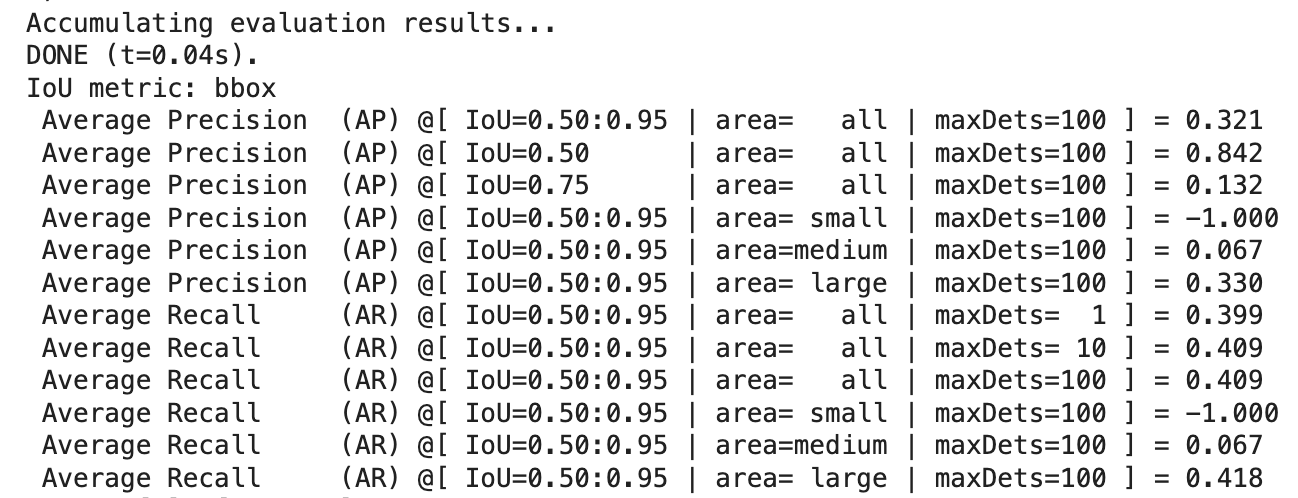
\includegraphics[width=\textwidth]{images/eval_coco_benchmark_white.png}
    \caption{Exemple de benchmark COCO dans la console}
    \label{fig:eval_coco_benchmark}
\end{figure}
La précision moyenne, (AP-Average Precision) présente dans les résultats COCO est calculée sur toutes les catégories, elle correspond traditionnellement au mean Average Precision (mAP).
Les résultats sont divisé en 4 catégories qui dépendent du score IoU ou de l'air de la bounding box prédite.
\begin{itemize}
    \item Les trois premières lignes sont l'AP en considérant différents seuil d'IoU pour sélectionner les boudings boxes à évaluer.
    \item Les trois suivantes sont l'AP en considérant des surfaces de tailles différentes pour sélectionner les boudings boxes à évaluer
    \item Les trois suivantes sont le Rappel Moyens (AR) en considérant plusieurs IoU pour sélectionner les boudings boxes à évaluer.
    \item Les trois suivantes sont l'AR en considérant des surfaces de tailles différentes pour sélectionner les boudings boxes à évaluer.
\end{itemize}
Selon la $\text{documentation}^1$, la première ligne est la plus importante. A la place de considérer les bounding boxes qui ont un IoU plus grand que le seuil, il est calculé sur cette ligne la moyenne des mAP des bounding boxes selon 10 seuils différents (de 0.5 à 0.95 par pas de 0.05).
%https://github.com/facebookresearch/detectron2/blob/main/MODEL_ZOO.md
Il faut noter que s'il n'existe pas de bounding boxes répondant aux critères, un score de \verb|-1| est affiché. On observe donc qu'il n'existe pas de bounding box de petite taille (32x32 pixels) puisque l'AP ainsi que l'AR où l'air est petite vaut \verb|-1|.
\paragraph{}
Avec Detectron2, un benchmark COCO est fait après chaque époch. C'est à dire lorsque le modèle à vu une fois le dataset en entier. Ce benchmark est effectué sur un fold du set d'entrainement appelé validation. Cependant, afin de véritablement tester les résutlats, nous avons aussi effectué un benchmark COCO sur un set de test d'images jamais vues par le modèle. 
Detectron2 sauvegarde les résultats dans un fichier json, ce fichier peut être lu par un widget TensorBoard afin de monitorer l'entrainement.
Les résultats peuvent aussi être visualisés de manière résumées, par défaut ce n'est pas fait durant l'entrainement uniquement lors d'un benchmark COCO complet. Le résumé s'affiche comme dans l'image \ref{fig:eval_coco_benchmark_resume} 
\begin{figure}
    \centering
    \scalebox{0.5}[0.5]{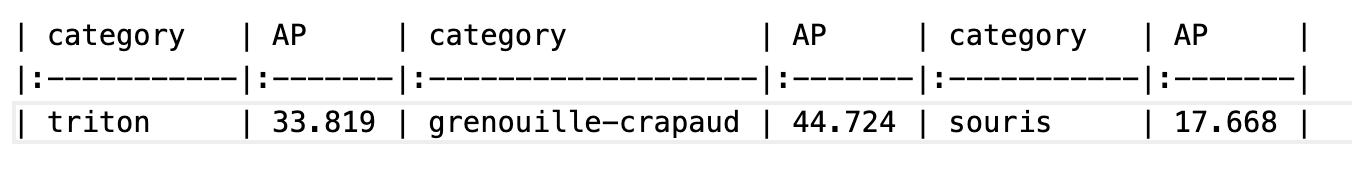
\includegraphics[width=\textwidth]{images/eval_coco_benchmark_resume.png}}
    \caption{Exemple de résumé COCO}
    \label{fig:eval_coco_benchmark_resume}
\end{figure}
On voit très facilement que les AP sont désormais calculés par classes sans distinction de IoU. 

\section{L'entrainement}\label{anal:train}
Nous avons entrainé les modèles un après l'autre sur un set de test composé de 176 tritons, 170 crapaud-grenouilles ainsi que de 150 souris. Ce dernier animal n'était pas demandé dans la tâche, mais nous nous sommes dit que ça permettrait d'ajouter de la diversité dans le dataset.
L'évaluation a été effectuée sur un set composé de 48 tritons, 47 crapaud-grenouilles et 30 souris. Les labels ont été fournis par le professeur.
Nous n'avons pas changé les paramètres généraux de Detectron2, uniquement les paramètres relatifs aux différents modèles, les entrainements se sont déroulés sur une GPU premium dont la spécification est visible dans le listing \ref{lst:gpu_spec}
\lstset{style=Bash}
\begin{lstlisting}[caption = {Résultat de la commande nvidia-smi},label={lst:gpu_spec}]
NVIDIA-SMI:     460.32.03    
Driver Version: 460.32.03    
CUDA Version:   11.2     
GPU  Name:      A100-SXM4-40GB
\end{lstlisting}
Les versions de Pytorch, ainsi que de python était celle par défaut sur colab au moment de l'entrainement.

\section{Tensorboard de faster RCNN }\label{anal:train_rcnn}
Les widgets tensorboard permettent durant tous les entrainements d'avoir un aperçu des différentes métriques enregistrées. Nous pouvons donc savoir quand arrêter l'entrainement pour avoir la meilleur performance selon une métrique, cela permet aussi de ne pas overfit. Nous avons pris quelques captures d'écrans affichées dans les figures \ref{fig:tensorboard_overview} et \ref{fig:tensorboard_metric}
\begin{figure}[h!]
    \centering
    \begin{subfigure}[t]{0.49\textwidth}
        \centering
        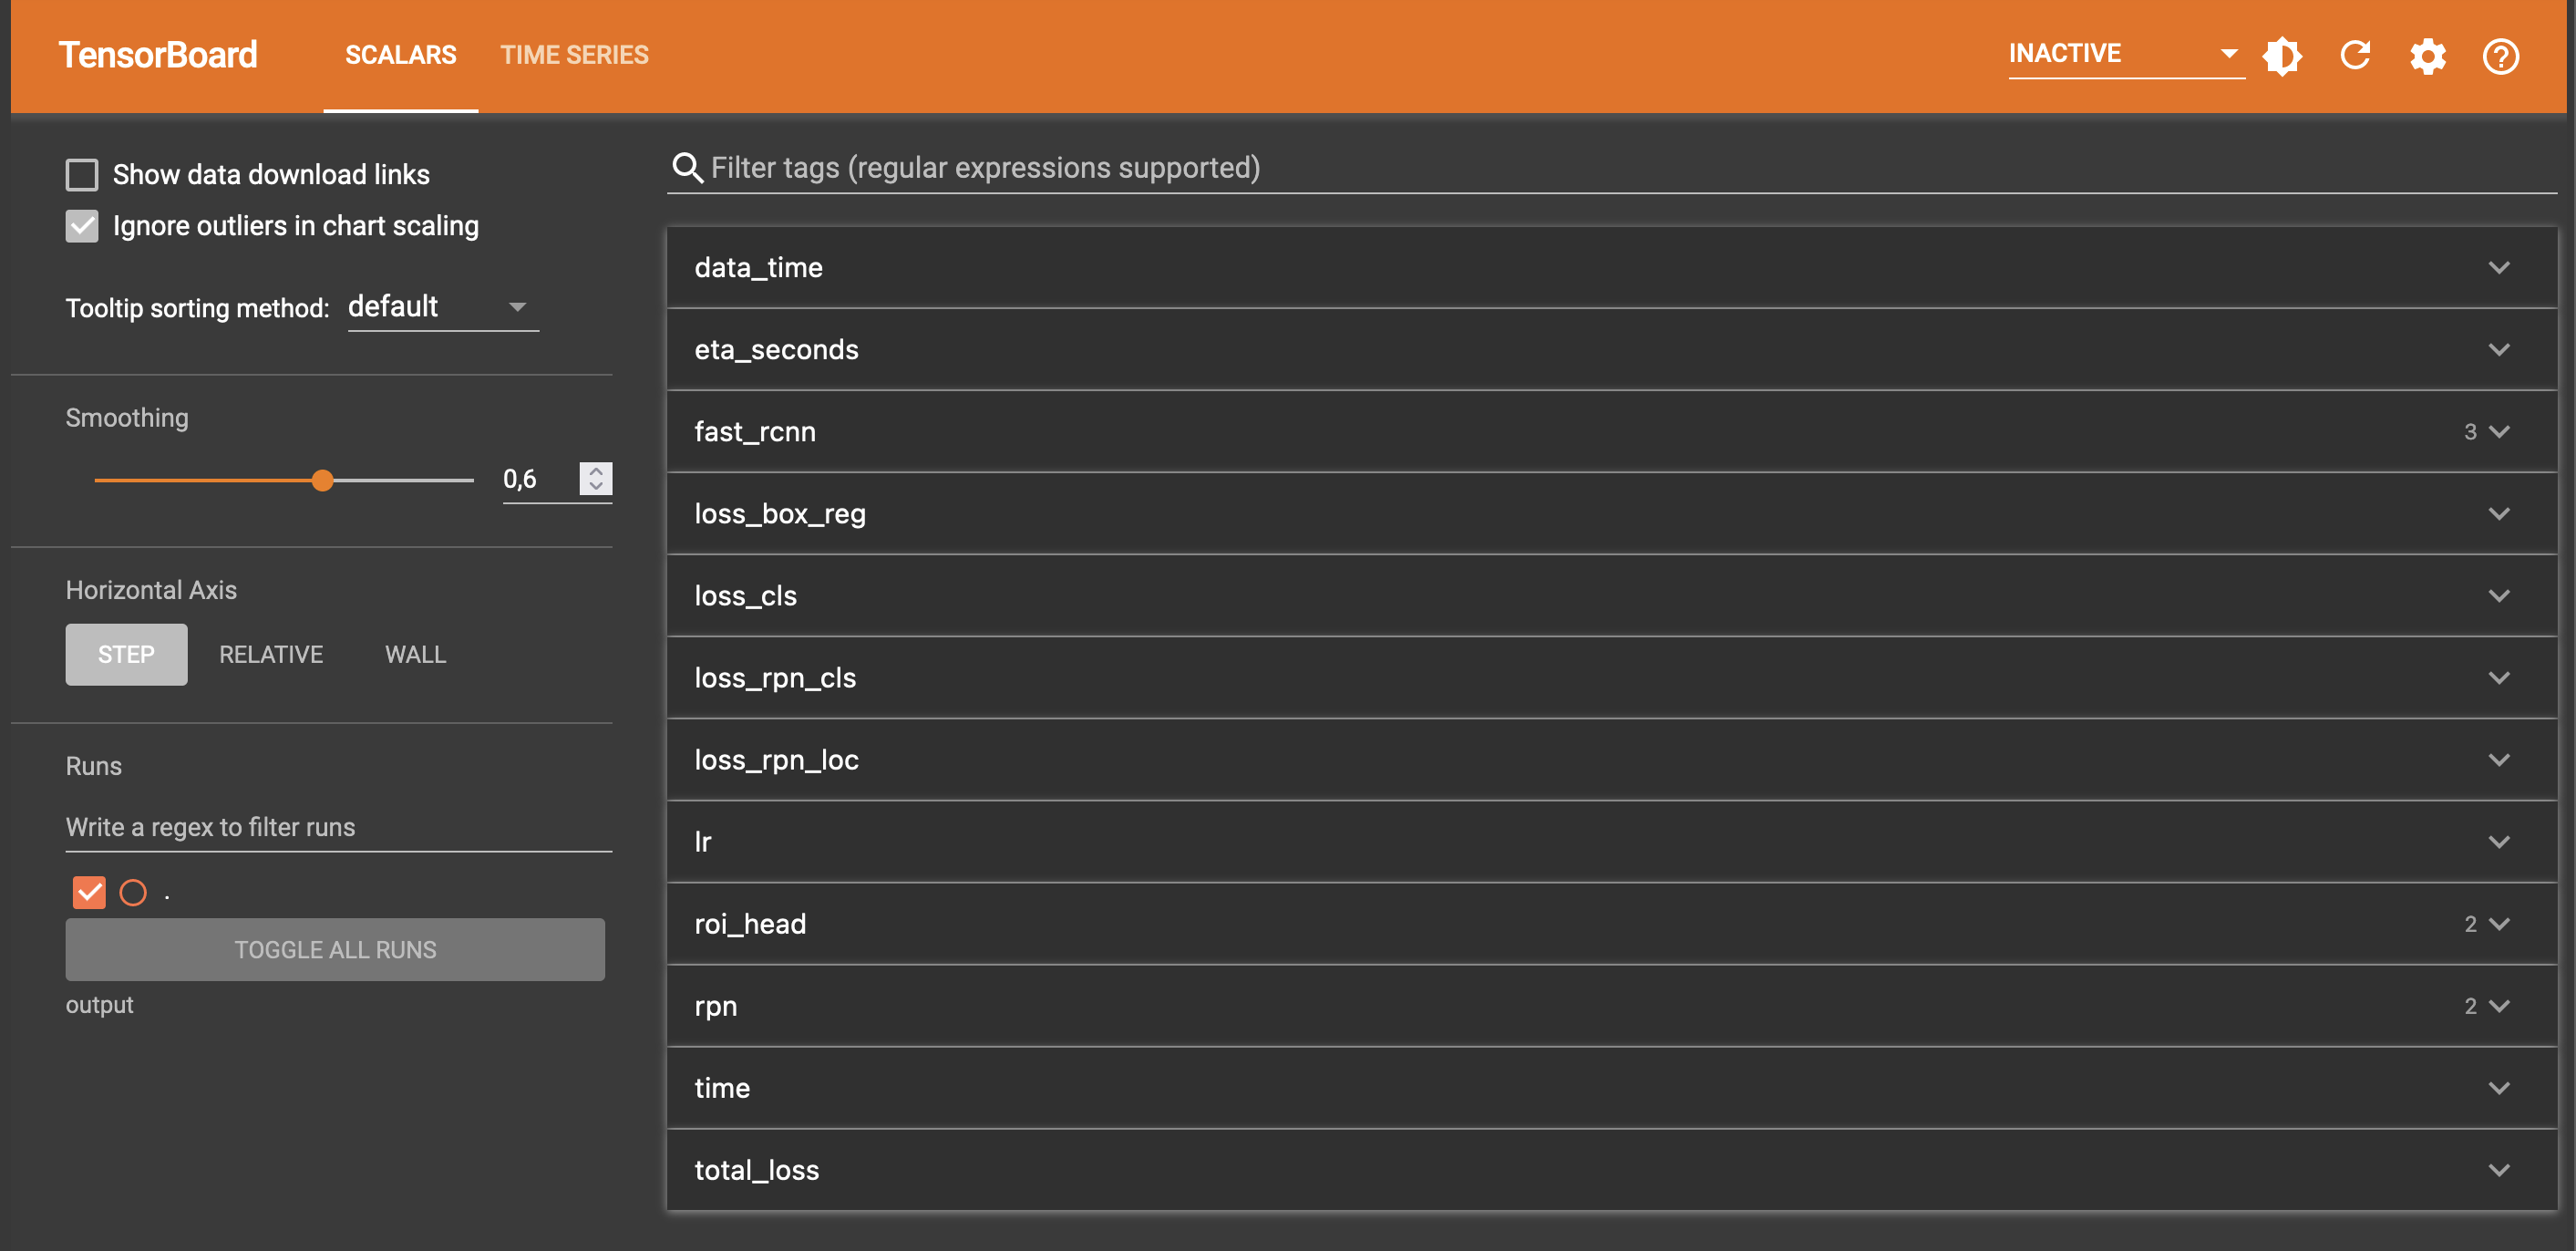
\includegraphics[width=\textwidth]{images/tensorboard_large.png}
        \caption{Aperçu du widget Tensorboard}
        \label{fig:tensorboard_overview}
    \end{subfigure}
    \begin{subfigure}[t]{0.49\textwidth}
        \centering
        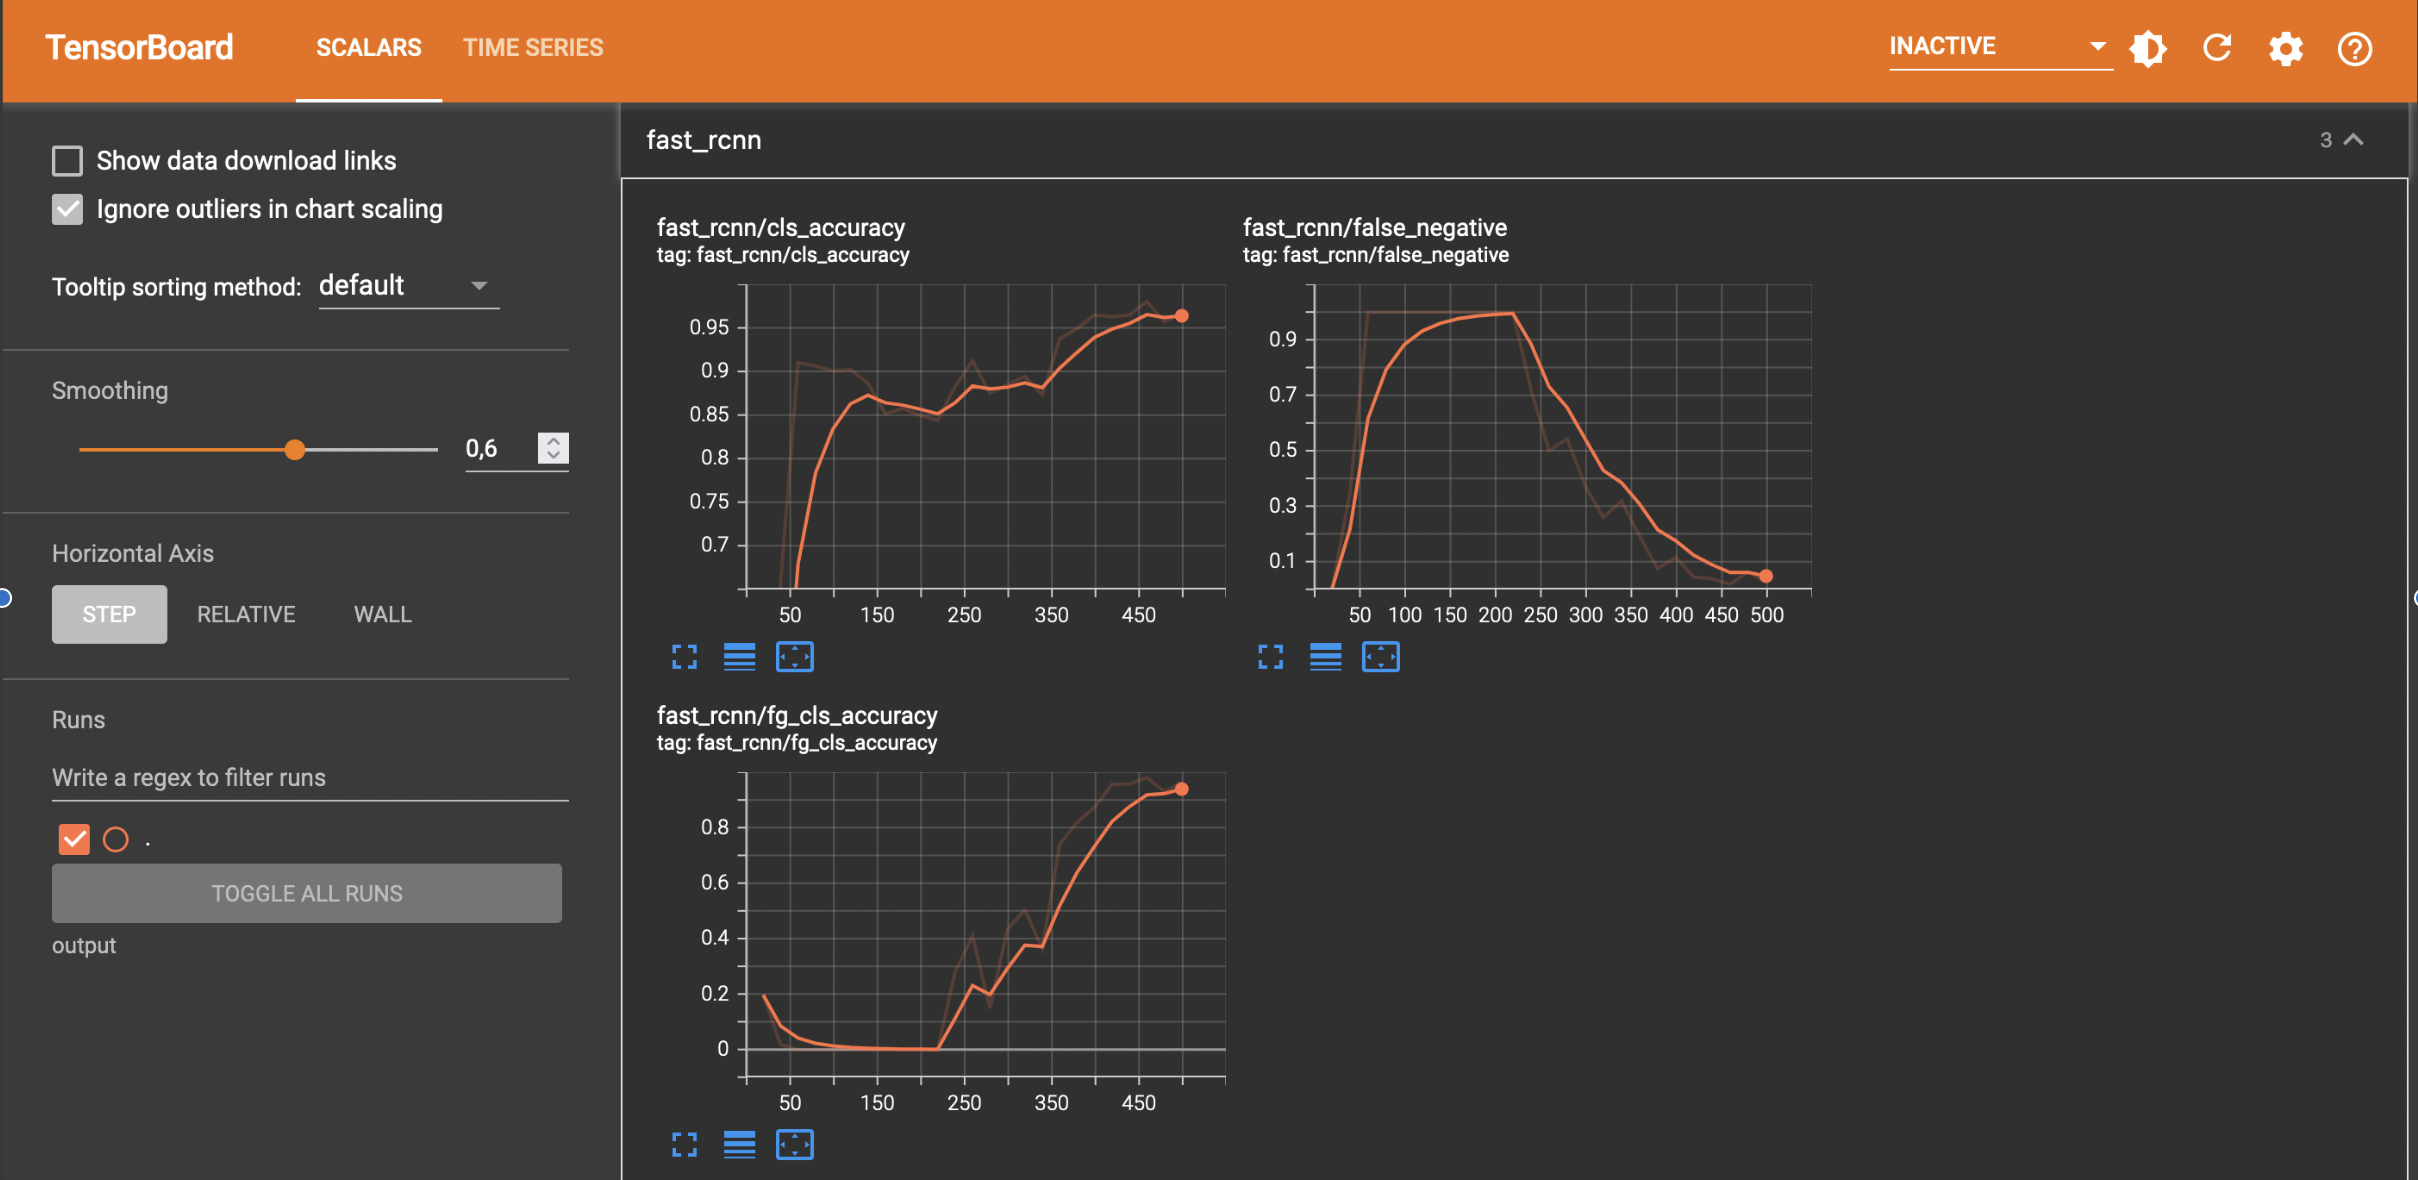
\includegraphics[width=\textwidth]{images/tensorboard_metric.png}
        \caption{Aperçu de cls\_accuracy, false\_negative et foreground\_cls\_accuracy durant l'entrainement.}
        \label{fig:tensorboard_metric}
    \end{subfigure}
    % \scalebox{0.5}[0.5]{}
    % \caption{Aperçu du widget Tensorboard}
    % \label{fig:tensorboard_overview}
    % \scalebox{0.5}[0.5]{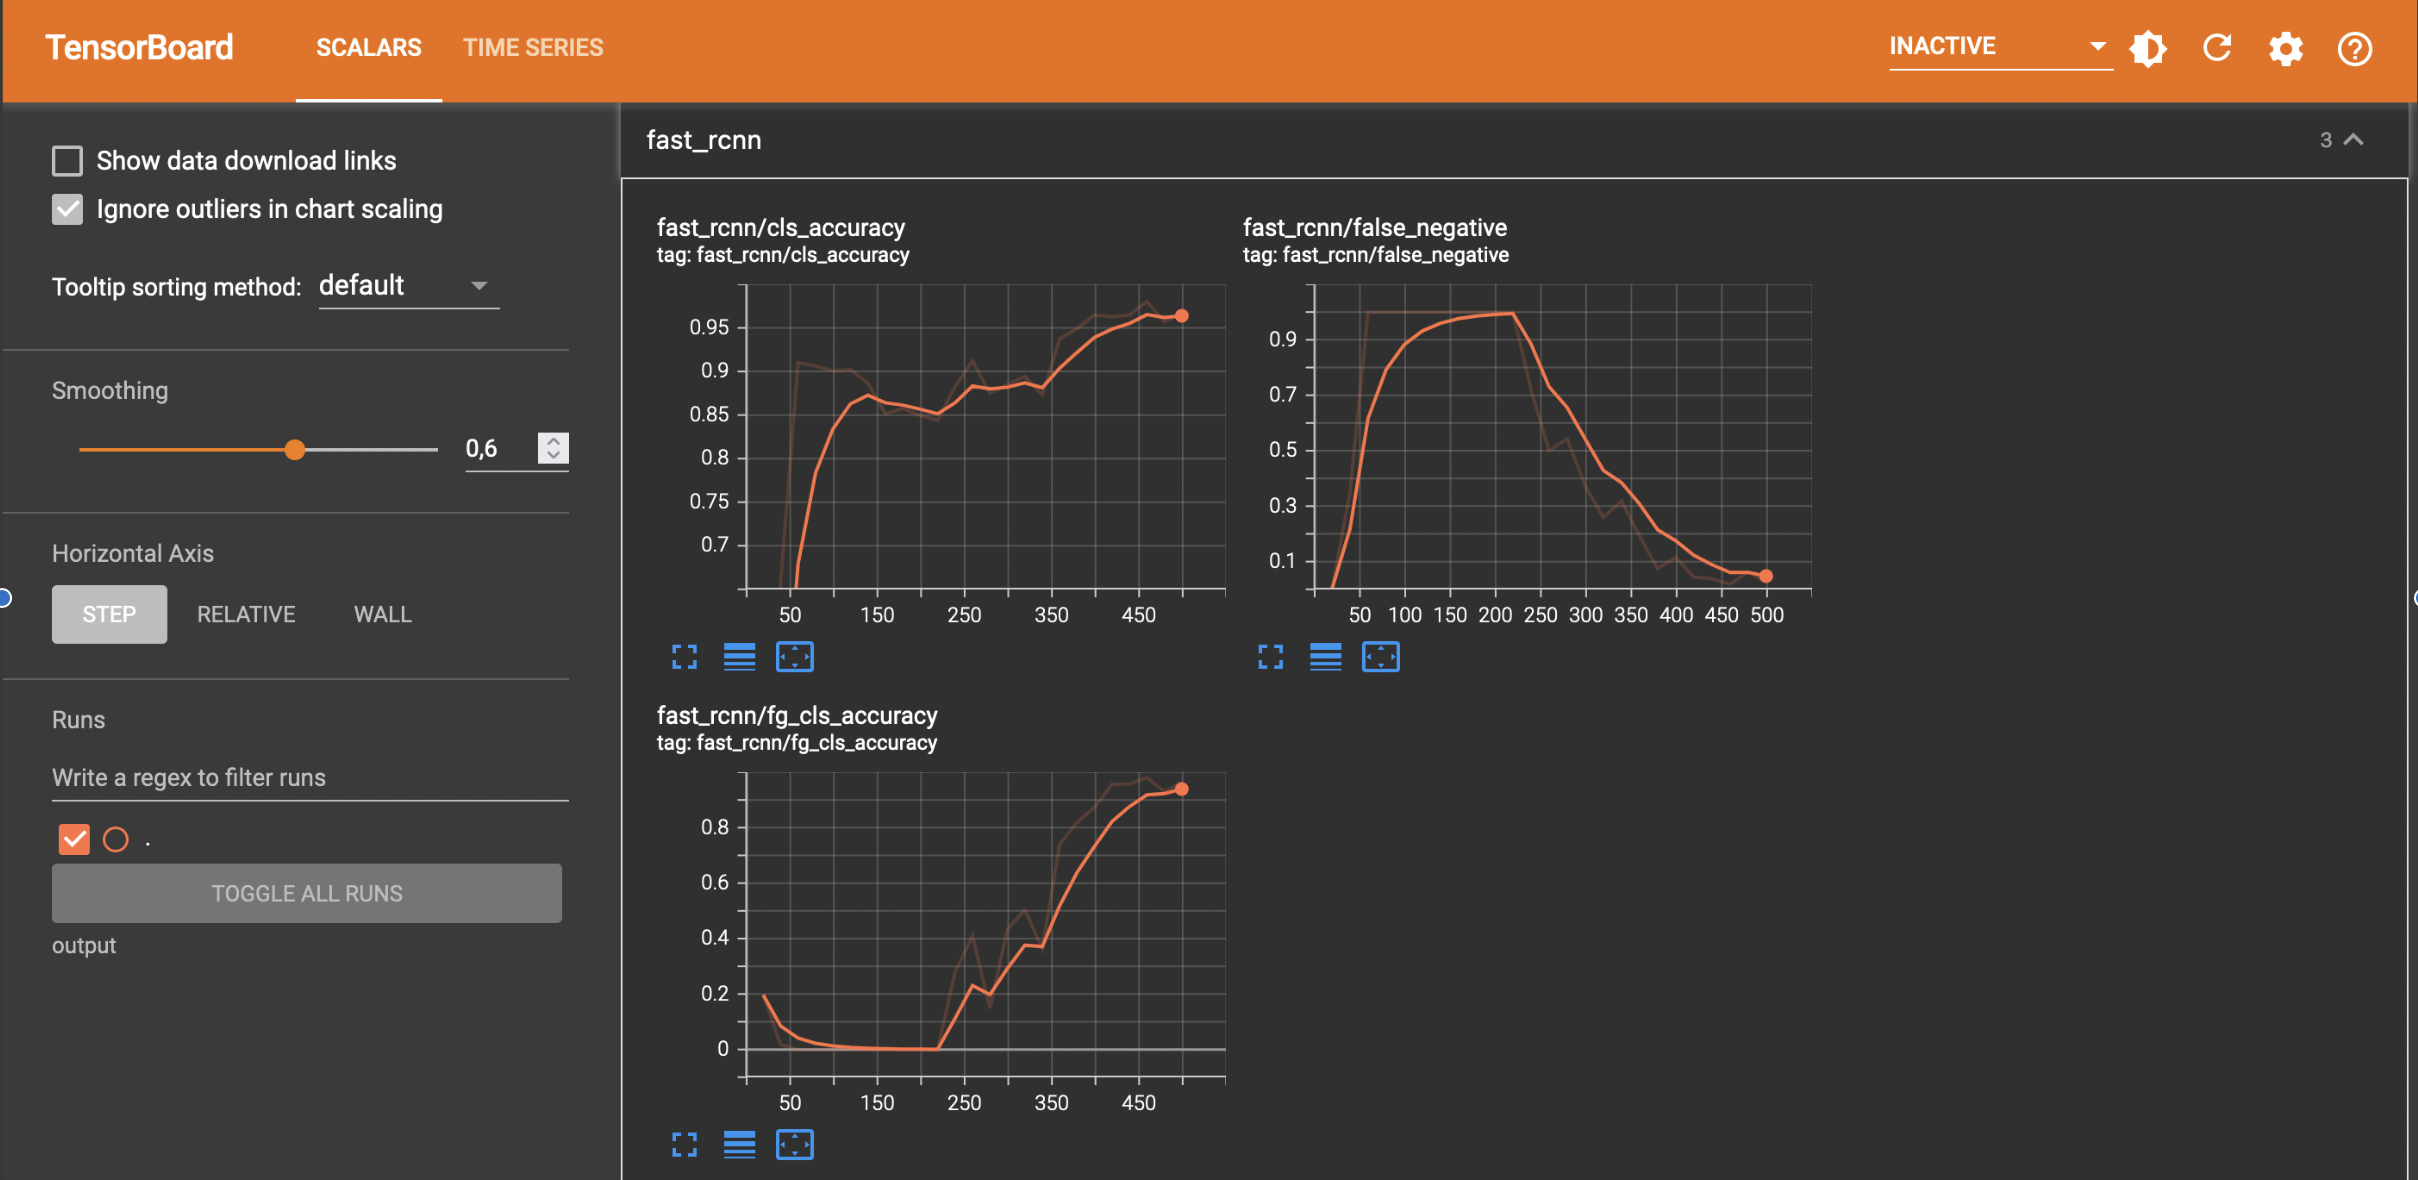
\includegraphics[width=\textwidth]{images/tensorboard_metric.png}}
    % \caption{Aperçu des métriques enregistrées dans TensorBoard}
    \caption{Aperçu de tensorboard et des métriques de faster RCNN}
\end{figure}
Detectron2 affiche aussi une loss total, nous n'avons pas réussis à déterminer la manière dont elle est calculée, mais elle reste un bon indicateur de la performance du model et de l'over/under fitting. De plus, comme nous avons plusieurs modèles, nous pouvons les comparer entre eux avec cette dernière puisques toute erreur sera identique sur tous les modèles, ainsi la comparation reste pertinente.
\begin{figure}[hb!]
    \centering
    \scalebox{0.5}[0.5]{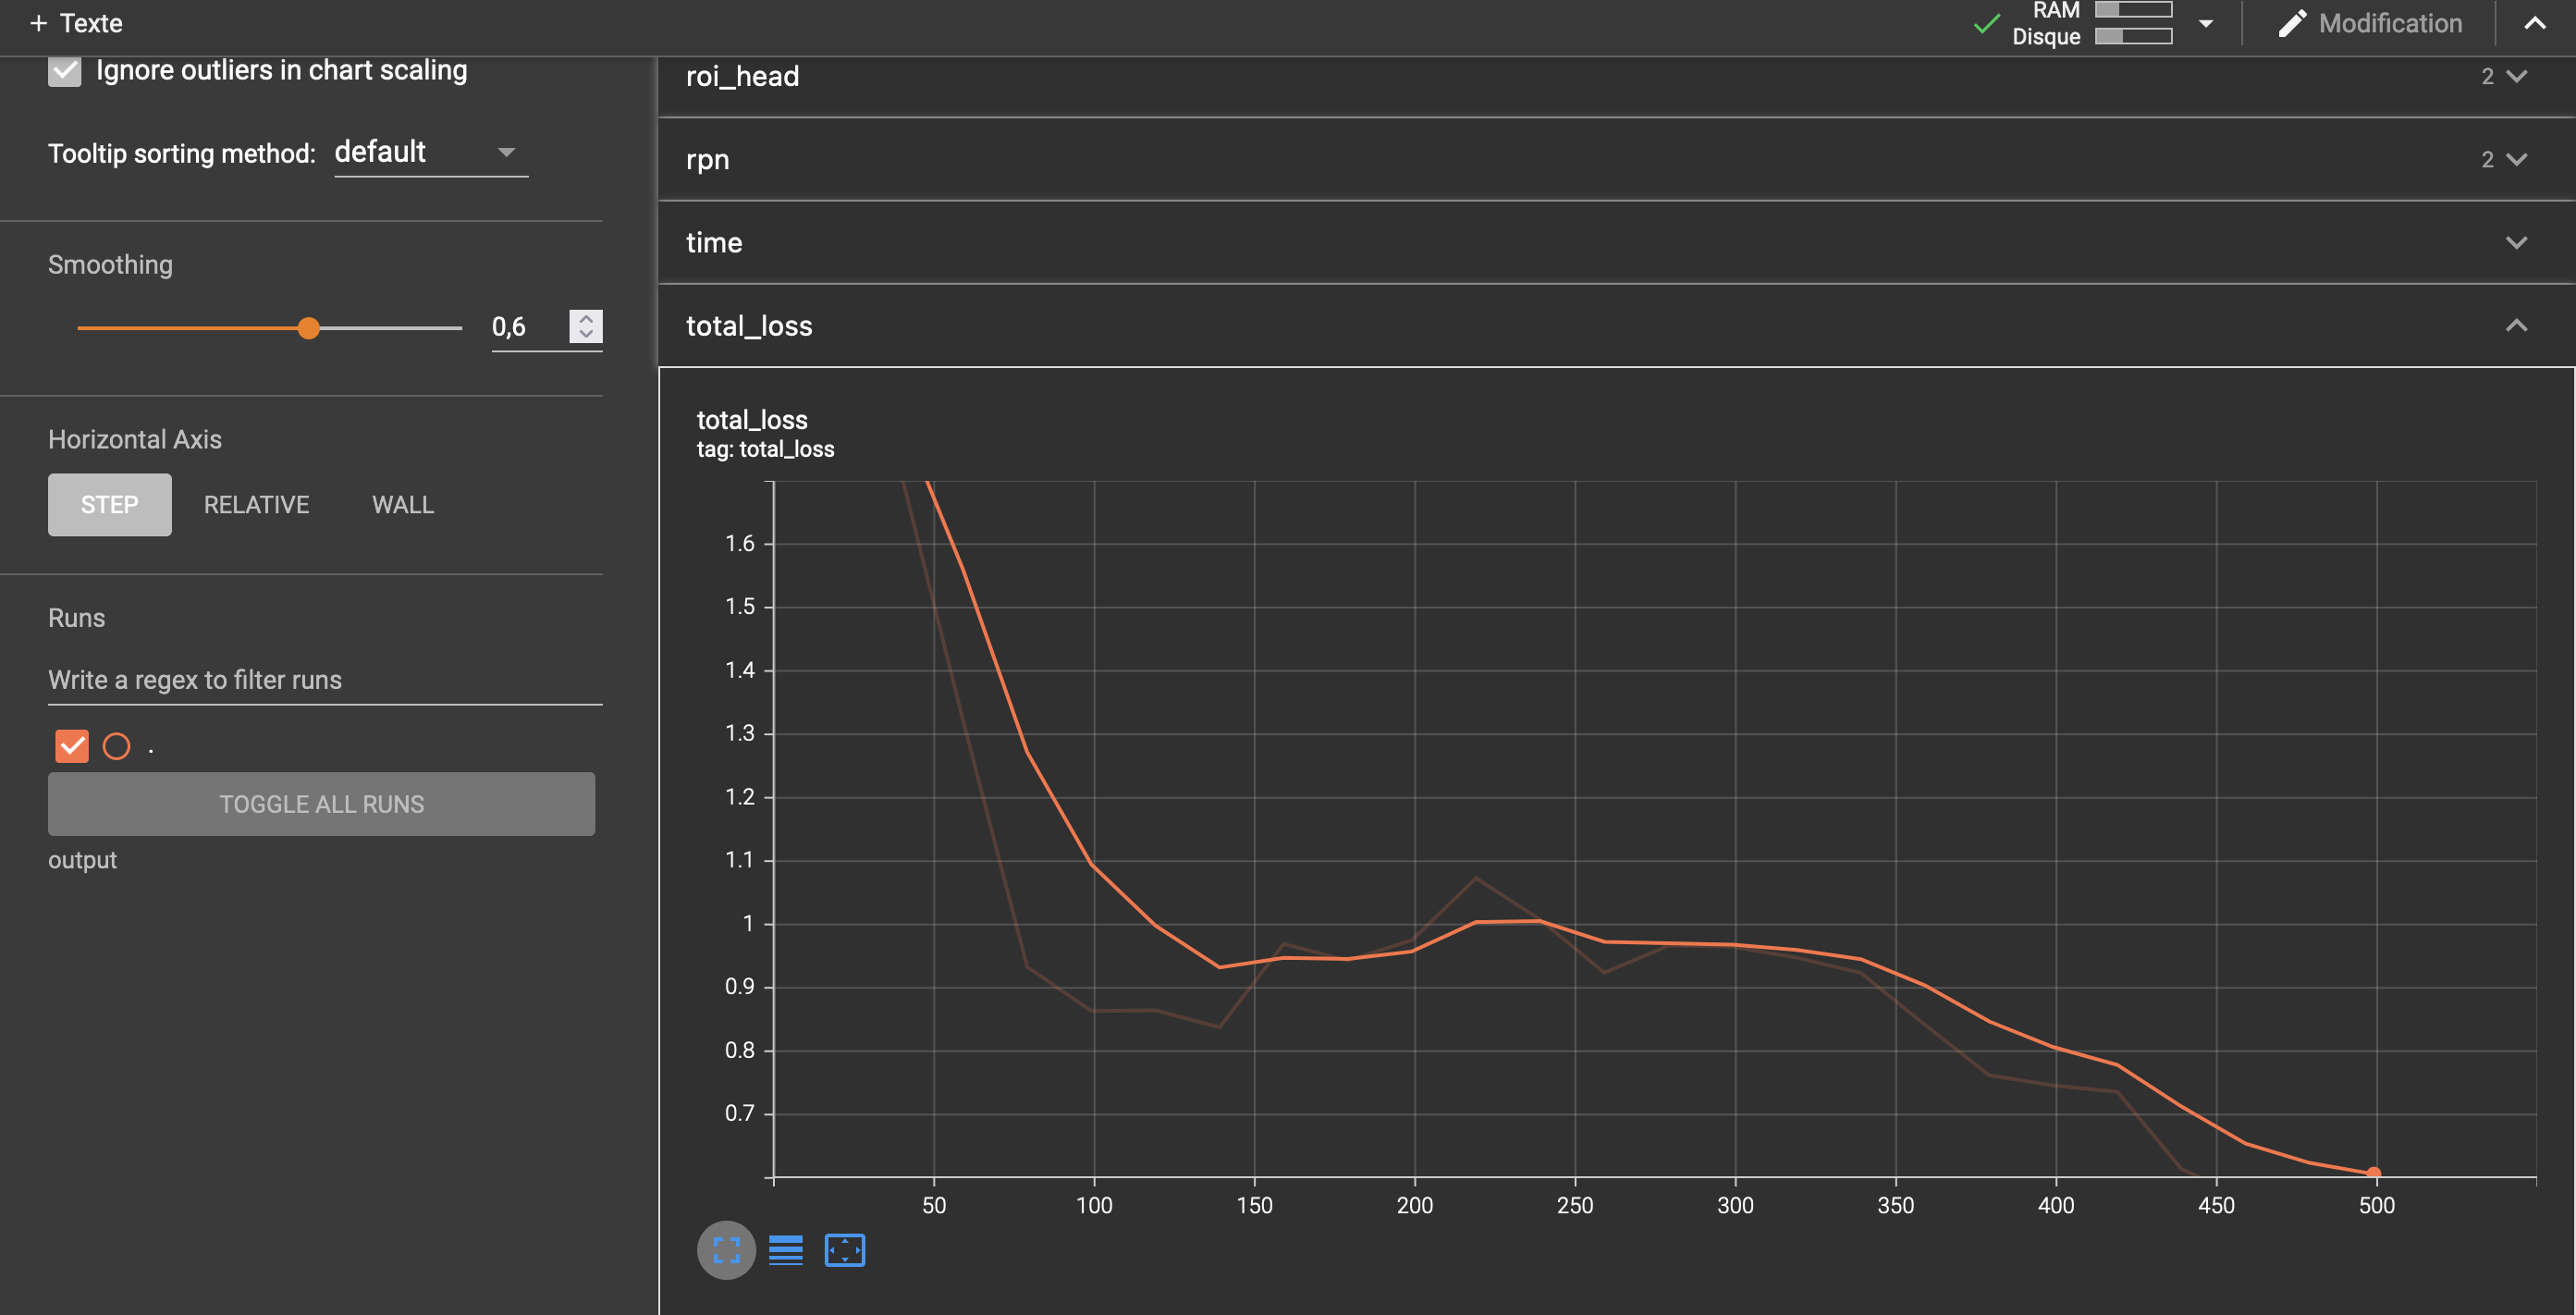
\includegraphics[width=\textwidth]{images/loss_faster_rcnn.png}}
    \caption{Aperçu de la loss total enregistrée dans TensorBoard}
    \label{fig:loss_faster_rcnn}
\end{figure}
Comme nous pouvons le voir dans la figure \ref{fig:loss_faster_rcnn}, nous n'avons ni d'overfit, ni d'underfit.


\section {Loss de RetinaNet}\label{anal:train_retina}
Dans cette section nous allons observer les métriques du modèle RetinaNet. Ce modèle enregistre moins de métriques, ceci est du au fait qu'il ne possède pas une architecture aussi complexe que Faster-RCNN. Alors que Faster-RCNN présentait des métriques pour certaines parties spécifiques du réseau, les RPN (Region Proposal Network) par exemple, RetinaNet ne présente que deux métriques relatives à l'entrainement : la loss de classification ainsi que la loss des bounding boxes.
\begin{figure}[h!]
    \begin{subfigure}[h]{0.49\textwidth}
        \centering
        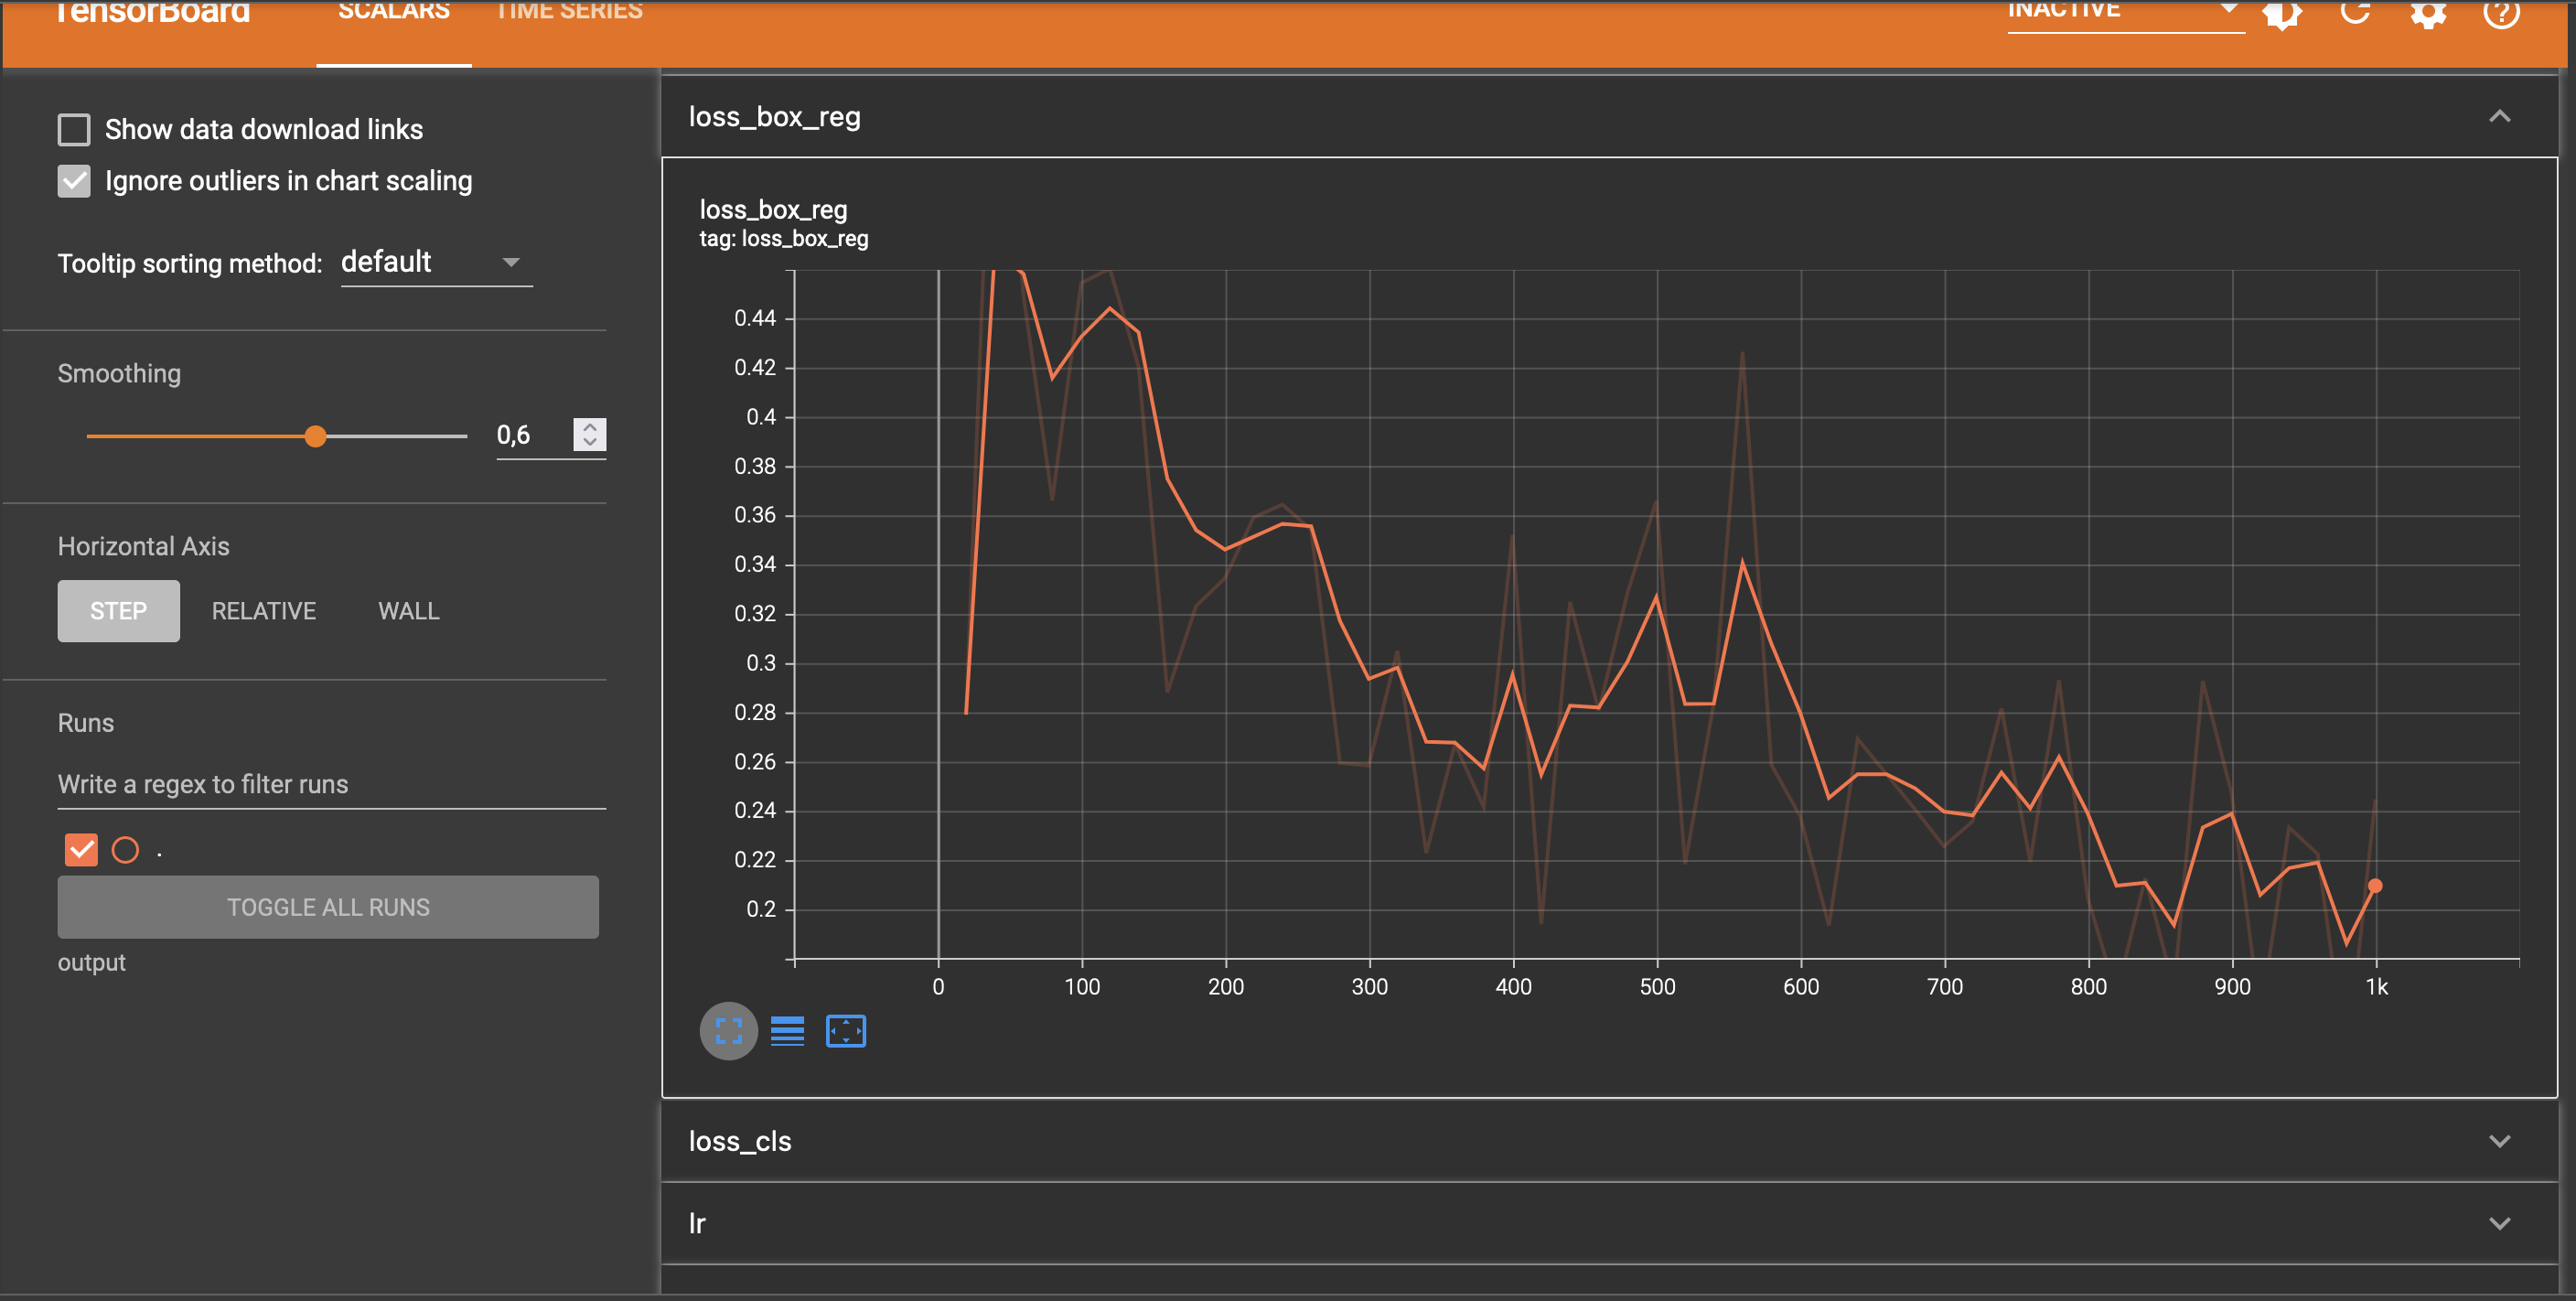
\includegraphics[width=\textwidth]{images/tensorboard_retina_net_loss_box.png}
        \caption{Loss des bounding boxes}
        \label{fig:loss_retinanet_box}
    \end{subfigure}
    \begin{subfigure}[h]{0.49\textwidth}
        \centering
        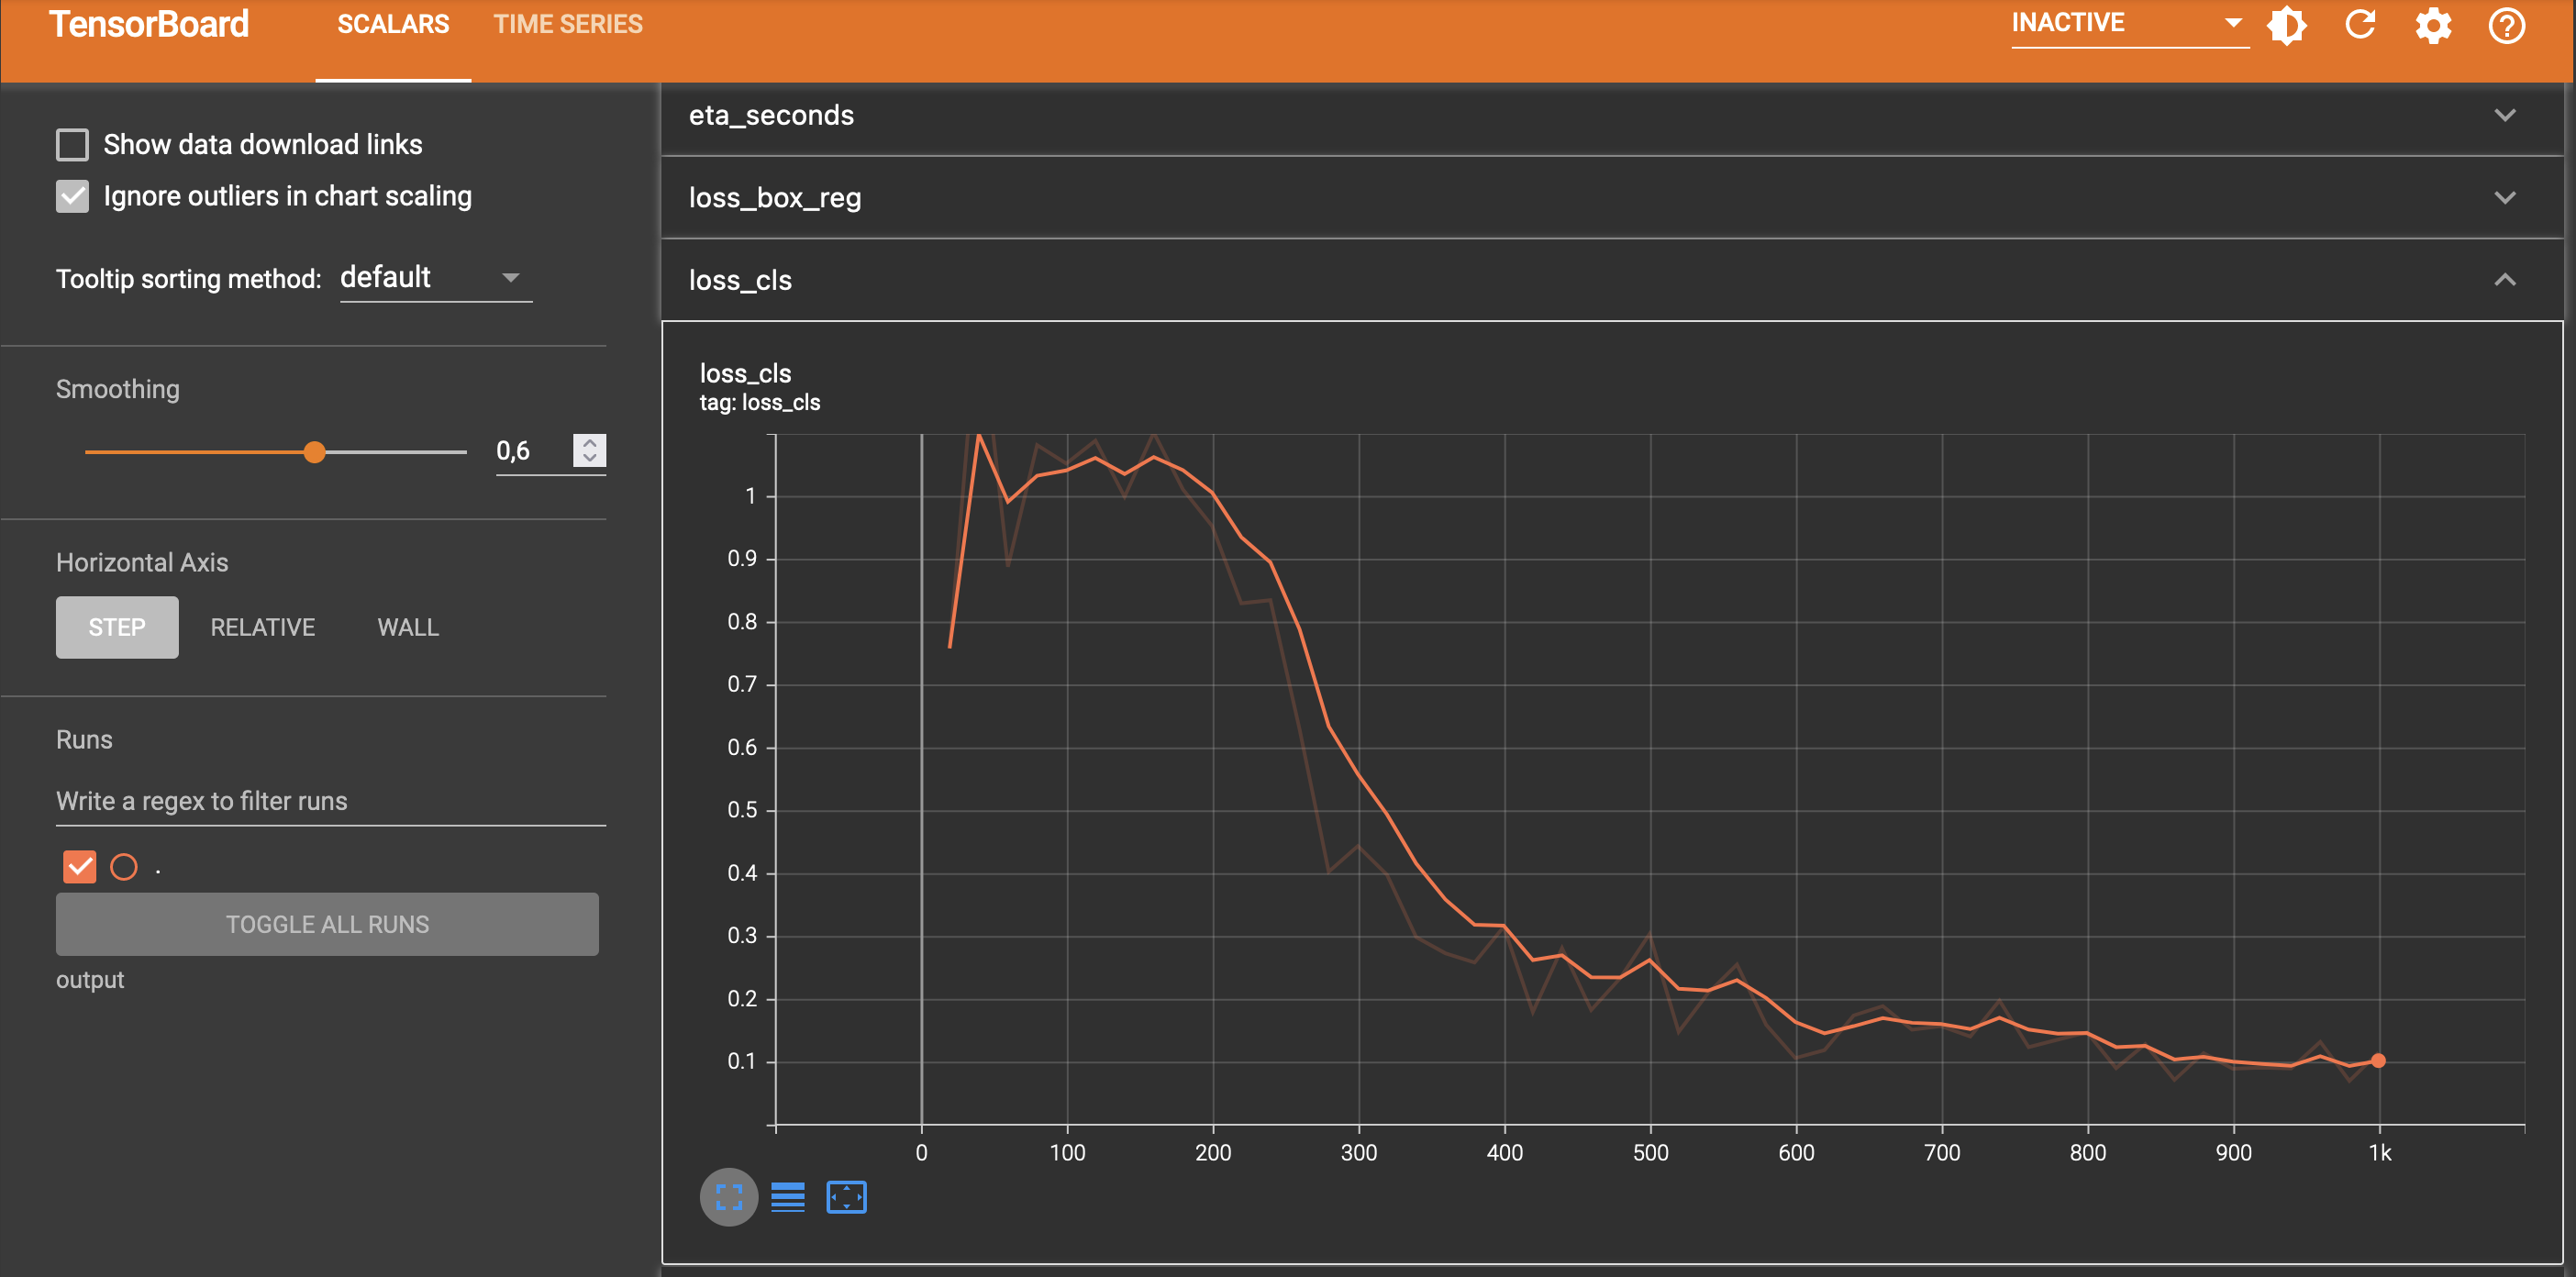
\includegraphics[width=\textwidth]{images/tensorboard_retina_net_loss_cls.png}
        \caption{Loss pour la classification}
        \label{fig:loss_retinanet_cls}
    \end{subfigure}
    \caption{Les métriques de RetinaNet durant un entrainement}
\end{figure}
Nous pouvons observer que RetinaNet doit être plus entrainé, 1000 itérations contre 500 pour Faster-RCNN. Il ne faut pas confondre itérations et époch. Une époch représente un passage sur l'entièreté du dataset, tandis qu'une iteration est un pas vers la recherche d'un minimum durant l'optimisation de l'erreur. Nous avons déterminé ces hyperparamètres grâce à tensorboard qui permet durant l'entrainement d'avoir un aperçu des métriques. Fait intéressant, RetinaNet est plus rapide à entrainer (environ 10 minutes de moins que Faster-RCNN) ceci est surement du à son architecture plus simple qui nécessite donc moins de calcule.

% -- Vic : 

\section{Évaluations des deux modèles sélectionnés}\label{anal:evaluation}

Après avoir testé plusieurs approches comme mentionnées dans le chapitre \ref{chap:Modeles}, nous avons retenu deux modèles dont nous allons ici comparer les scores d'évaluation :

\begin{itemize}
    \item[-] Faster R-CNN avec Detectron2 et
    \item[-] Retinanet avec Detectron2.
\end{itemize}

\subsection{Scores des modèles}

Voici donc les scores obtenus avec Faster R-CNN (figure \ref{fig:scores_fasterRcnn}) et RetinaNet (figure \ref{fig:scores_retinanet}) :

\begin{figure}[H]
    \centering
    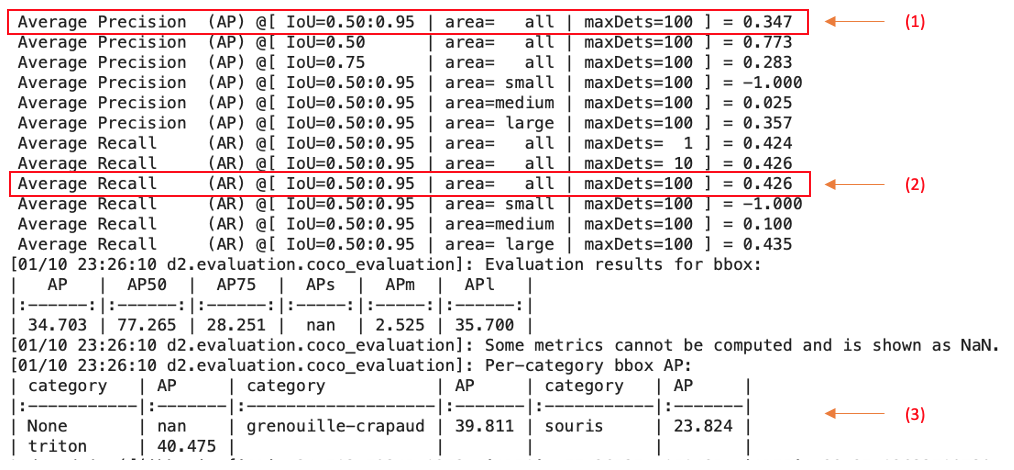
\includegraphics[width=\textwidth]{images/eval_FasterRCNN_resume_annote.png}
    \caption{Scores obtenus avec Faster R-CNN}
    \label{fig:scores_fasterRcnn}
\end{figure}

\begin{figure}[H]
    \centering
    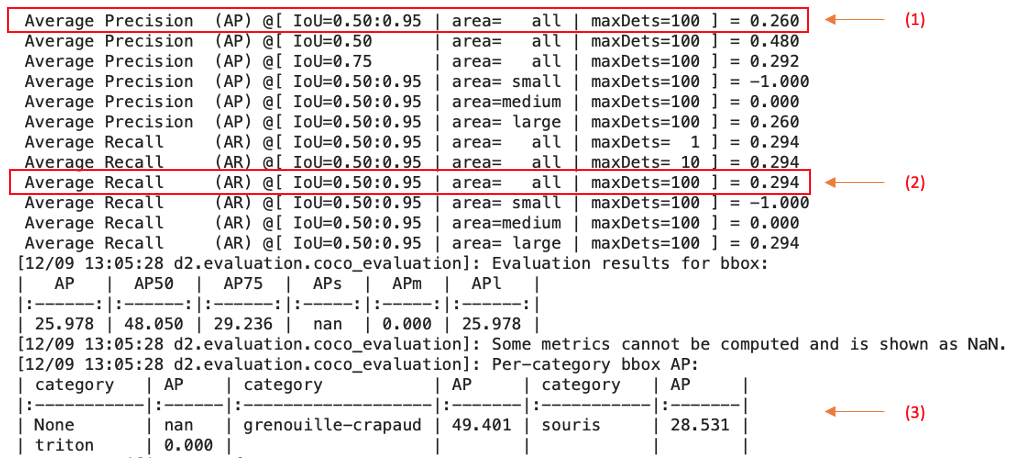
\includegraphics[width=\textwidth]{images/eval_Retinanet_resume_annote.png}
    \caption{Scores obtenus avec RetinaNet}
    \label{fig:scores_retinanet}
\end{figure}

D'après le chapitre 7.2 vu plus tôt "Lecture d'un benchmark COCO", c'est la première ligne de ces résultats qui est la plus importante, c'est-à-dire la moyenne des mAP des bounding boxes qui ont un IoU entre 50 et 95 pourcent. On va donc ici observer ces valeurs, ainsi que l'average recall recall pour le même intervalle de IoU, avec la même valeur (=100) pour maxDets - nombre maximal d'objets détectables sur une image. On peut observer ces valeurs sur les figures \ref{fig:scores_fasterRcnn} et \ref{fig:scores_retinanet}, en \textit{(1)} pour l'AP et en \textit{(2)} pour l'AR ; les voicis dans ce tableau :

\begin{center}
   \begin{tabular}{ | l || c | c |}
     \hline
     modèle & average precision & average recall \\ \hline
     Faster R-CNN & 0.347 & 0.426 \\ \hline
     Retinanet & 0.260 & 0.294 \\ \hline
   \end{tabular}
 \end{center}

On voit donc premièrement que les deux scores sont meilleurs pour Faster R-CNN que pour RetinaNet. Aussi, en observant les AP par classe (\textit{(3)} sur les figures \ref{fig:scores_fasterRcnn} et \ref{fig:scores_retinanet}), on a les résultats suivants : 

\begin{center}
   \begin{tabular}{ | l || c | c |}
     \hline
     modèle & AP grenouille-crapaud & AP triton \\ \hline
     Faster R-CNN & 39.811 & 40.475 \\ \hline
     Retinanet & 49.401 & 0.000 \\ \hline
   \end{tabular}
 \end{center}
 
On voit ici que bien que le score pour la classe crapaud-grenouille soit plus élevé à l'aide du modèle RetinaNet, le score pour la classe triton est de zéro. Rappelons que la tâche initiale de ce projet est de compter le nombre de triton/crapaud-grenouille qui utilisent les crapauduc ; ainsi, nous avons choisi l'algorithme Faster R-CNN comme modèle final pour cette tâche de classification.\newline

Il est également ici intéressant de noter que le fait que la classe triton ait une AP nulle avec RetinaNet a un impact important sur le résultat de mAP. Il serait dont important et intéressant d'investiguer plus profondément sur la raison de l'échec complet de détection de triton ; comme discuté plus tard au \ref{chap:next_steps} de ce rapport.

\subsection{Modèle final choisi}\label{anal:final_model}

\paragraph{Entraînement}

Voici donc comment nous avons premièrement entraîné notre modèle Faster R-CNN, avec Detectron 2 : 

\lstset{language=Python}
\lstset{style=Python}
\begin{lstlisting}
cfg = get_cfg()
cfg.merge_from_file(model_zoo.get_config_file("COCO-Detection/
faster_rcnn_X_101_32x8d_FPN_3x.yaml"))
cfg.DATASETS.TRAIN = ("triton_train",)
cfg.DATASETS.TEST = ()
cfg.DATALOADER.NUM_WORKERS = 2
cfg.MODEL.WEIGHTS = model_zoo.get_checkpoint_url("COCO-Detection/
faster_rcnn_X_101_32x8d_FPN_3x.yaml")  
cfg.SOLVER.IMS_PER_BATCH = 2 
cfg.SOLVER.BASE_LR = 0.00020 
cfg.SOLVER.MAX_ITER = 500 
cfg.SOLVER.STEPS = []   
cfg.MODEL.ROI_HEADS.BATCH_SIZE_PER_IMAGE = 128  
cfg.MODEL.ROI_HEADS.NUM_CLASSES = 4 
\end{lstlisting}


\paragraph{Test}

Et voici donc le modèle construit pour tester nos données d'évaluation : 

\lstset{style=Python}
\begin{lstlisting}
# on recuperation des poids du modele qu'on vient d'entrainer
cfg.MODEL.WEIGHTS = os.path.join(cfg.OUTPUT_DIR, "model_final.pth")  
# determination d'un treshold pour le test
cfg.MODEL.ROI_HEADS.SCORE_THRESH_TEST = 0.7  
# construction du predicteur
predictor = DefaultPredictor(cfg)
\end{lstlisting}

Le treshold choisi pour le test ci-dessus indique donc qu'on considérera une image comme étant prédite d'une certaine classe si le modèle est sûr à au moins 70\% de sa classification.\newline

Voici deux exemples de résultats de classification par notre modèle ainsi créé :

\begin{figure}[H]
    \centering
    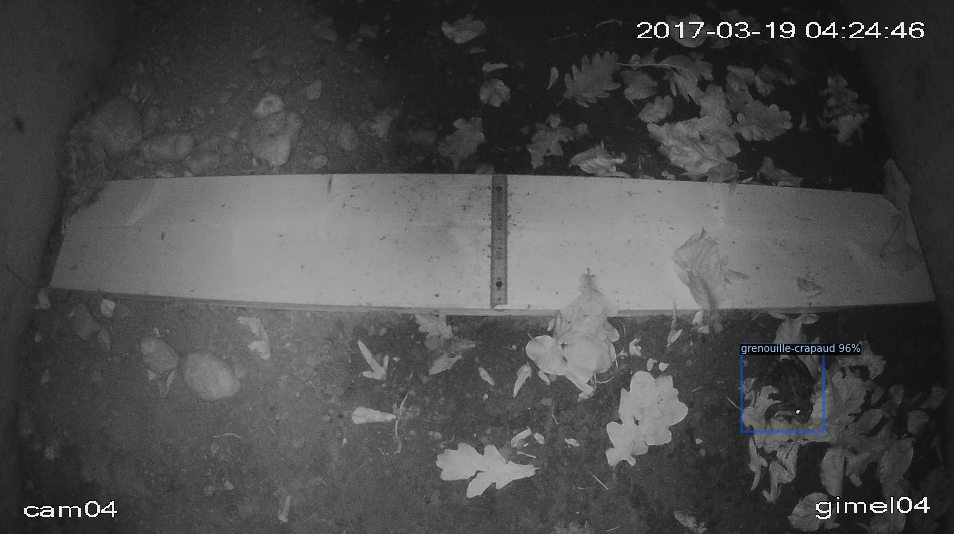
\includegraphics[width=300px]{images/Eval_FasterRCNN_crapGren.png}
    \caption{Prédiction de Faster R-CNN - crapaud-grenouille}
    \label{fig:fasterRcnn_crapGren}
\end{figure}

\begin{figure}[H]
    \centering
    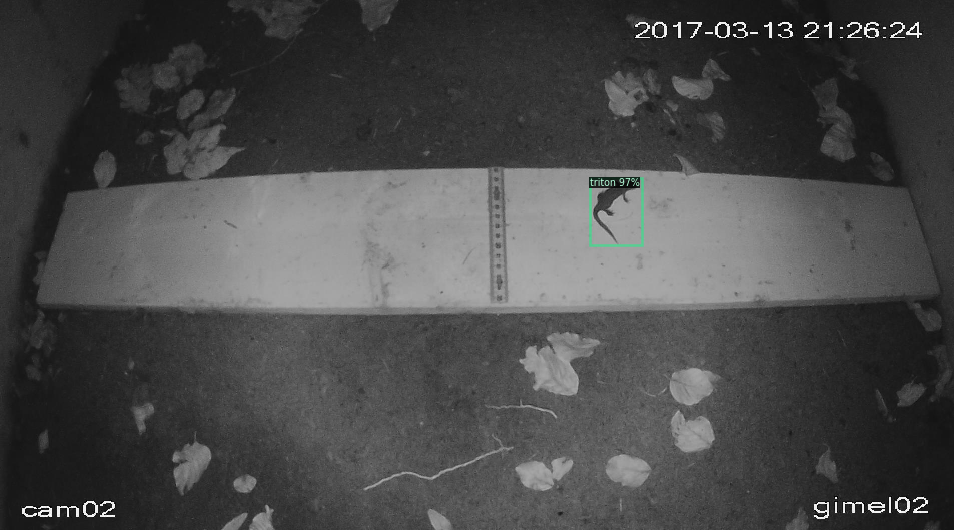
\includegraphics[width=300px]{images/Eval_FasterRCNN_triton.png}
    \caption{Prédiction de Faster R-CNN - triton}
    \label{fig:fasterRcnn_triton}
\end{figure}

On observe donc ici une bonne prédiction du modèle, qui est quasi certain de son classement (96\% et 97\%). Il est cependant intéressant et surtout important de noter que le modèle a été entraîné sur des images qui peuvent être très semblables aux/à certaines images de celles sur lesquelles il a été évalué ensuite. En effet, les images que nous avons prises pour l'entraînement et pour l'évaluation proviennent d'un ensemble d'images pouvant provenir de la même séquence ou du même crapauduc, ce qui peut provoquer de l'overfitting.

\section{Où est le problème}\label{ch:eval:sex:problem}

Nous avons donc des résultats qui approchent ceux de l'état de l'art en 2019 selon \url{https://paperswithcode.com/sota/object-detection-on-coco}. Nous avons aussi des modèles qui sont correctement entrainés puisque, nous l'avons vu dans la partie \ref{anal:train_rcnn} ainsi que \ref{anal:train_retina}, les métriques indiquent qu'ils sont ni sous-entrainés ni sur-entrainés. Il nous faut donc observer des mauvaises classifications afin de comprendre les erreurs et déterminer d'autres facteurs sur lesquels nous pouvons agir afin d'avoir de meilleurs résultats. En effet, à l'heure où nous écrivons ces mots, un modèle basé sur DETR \footnote[1]{\url{https://arxiv.org/pdf/2211.03594v1.pdf}} atteint 64.5 de mAP sur le benchmark COCO, ce qui est un score très élevé. Il existe donc des modèles SOTA bien meilleurs mais nous n'arrivons pas à les reproduire. Nous allons donc observer les erreurs de classification afin de comprendre ce qui ne va pas, mais avant nous aimerions faire remarquer qu'une explication possible est simplement la taille du Modèle. DETR, notre plus gros modèle, a 60 millions de paramètres alors que leur modèle en a 600 millions.
\subsection{Analyse des images non détectés par Faster-RCNN}
\begin{figure}[h]
    \centering
    \begin{subfigure}[h]{0.49\textwidth}
        \centering
        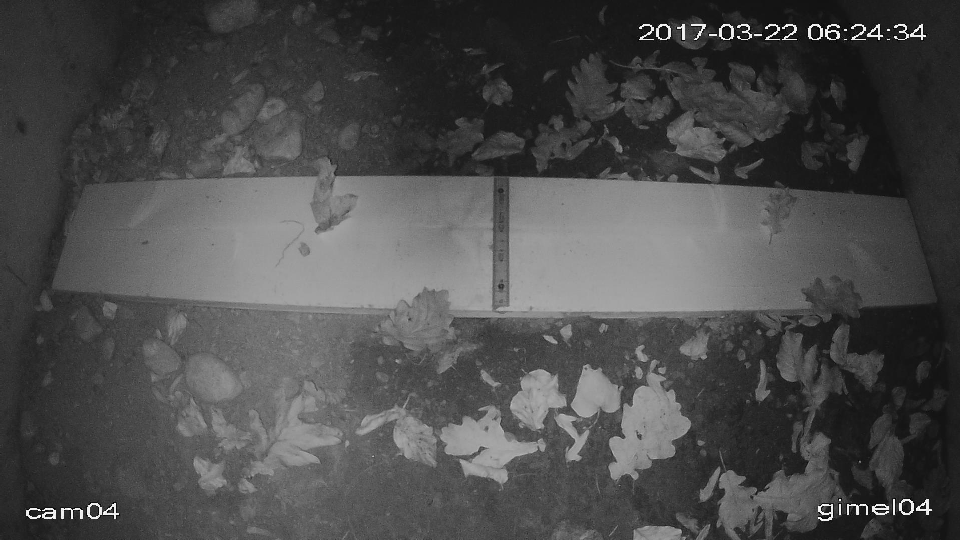
\includegraphics[width=0.9\textwidth]{images/failed_pred1_rcnn.png}
        \caption{Crapaud-grenouille caché}
        \label{fig:eval_fasterRCNN_a}
    \end{subfigure}
    \begin{subfigure}[h]{0.49\textwidth}
        \centering
        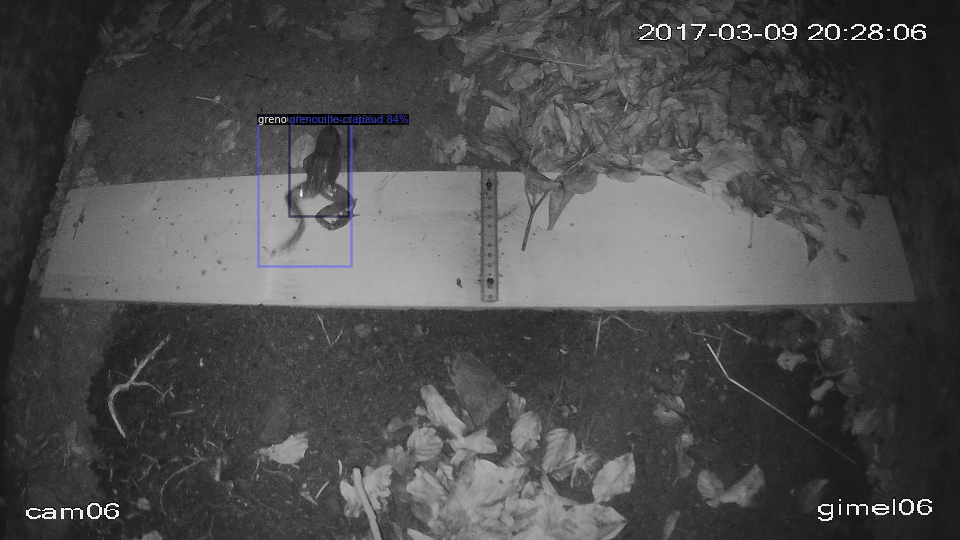
\includegraphics[width=0.9\textwidth]{images/failed_pred3_rcnn.png}
        \caption{Double bounding box}
        \label{fig:eval_fasterRCNN_b}
    \end{subfigure}
    \begin{subfigure}[h]{0.7\textwidth}
        \centering
        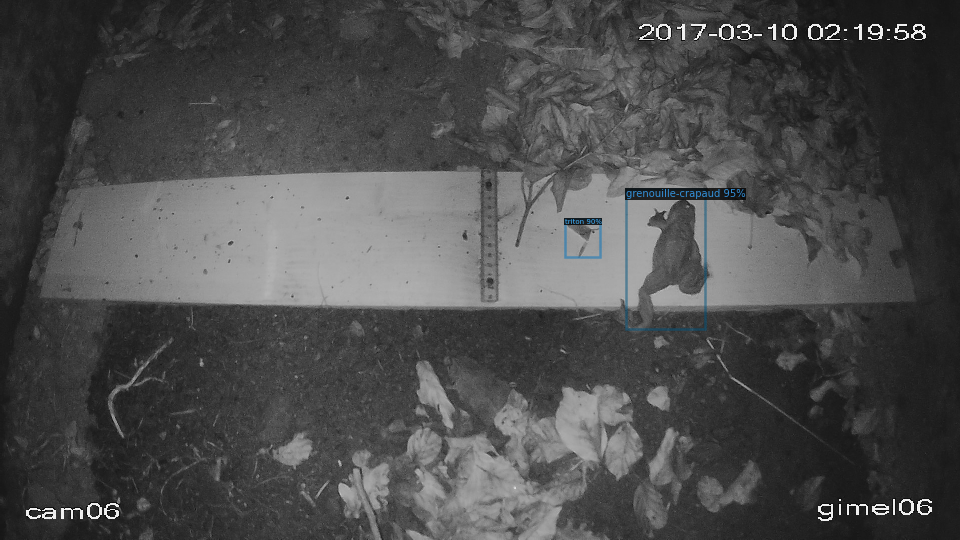
\includegraphics[width=0.9\linewidth]{images/failed_pred5_rcnn.png}
        \caption{Erreur de classification}
        \label{fig:eval_fasterRCNN_c}
    \end{subfigure}
    \caption{Exemple d'images mal prédites par Faster-RCNN}
    \label{fig:failed_pred_rcnn}
\end{figure}
La plupart des images qui présentent des erreurs pouvant expliquer le score de de Faster-RCNN ressemble aux images de la figure \ref{fig:failed_pred_rcnn}. 
Nous avons ici trois types d'erreurs. 
\paragraph{}
La première, qui est aussi une des plus fréquente, est la non détection d'animaux (souvent sur les bords de l'image). Le manque de luminosité ou la présence de feuille pourrait expliquer cela. Un pré-processing pourrait vérifier l'hypothèse de la luminosité. Cependant, nous ne pouvons pas vraiment faire de pré-processing pour la présence de feuille.
\paragraph{}
La seconde est aussi assez fréquente, il s'agit de la présence de multiples bounding boxes sur un même animal. Même si c'est étonnant, cette erreur ne devrait pas affecter les scores sur le benchmark. Nous avons aussi tuner le threeshold de confiance pour réduire ce genre d'erreur.
\paragraph{}
La dernière est la seul occurence de ce type observée sur le set de teste, on peut voir qu'un bout de feuille est mal classifié avec pourtant une probabilité de 90\%. Et ceci sans raisons visibles.
%  Nous pouvons nous demander si la planche à vraiment été bénéfique, en effet la plupart des annotations sont sur la planche, là où la planche permet rapidment d'apercevoir un animal. Le modèle a peut-être appris qu'il est plus probable de voir un animal donc peut-être plus habitué à voir des animaux à cet endroit.
En conclusion, Faster-RCNN est vraiment bon et les erreurs ne présentent pas de grâves erreurs d'entrainement.

\subsection{Analyse des images non détectés par RetinaNet}
\begin{figure}[H]
    \centering
    \begin{subfigure}[h]{0.49\textwidth}
        \centering
        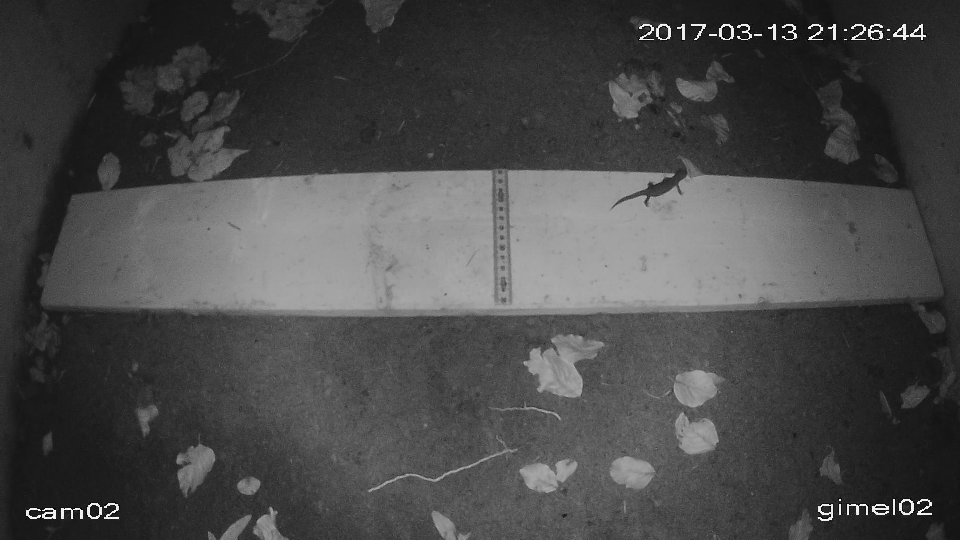
\includegraphics[width=0.9\textwidth]{images/failed_pred3_retina.png}
        \caption{Triton jamais détecté}
        \label{fig:eval_retina_a}
    \end{subfigure}
    \begin{subfigure}[h]{0.49\textwidth}
        \centering
        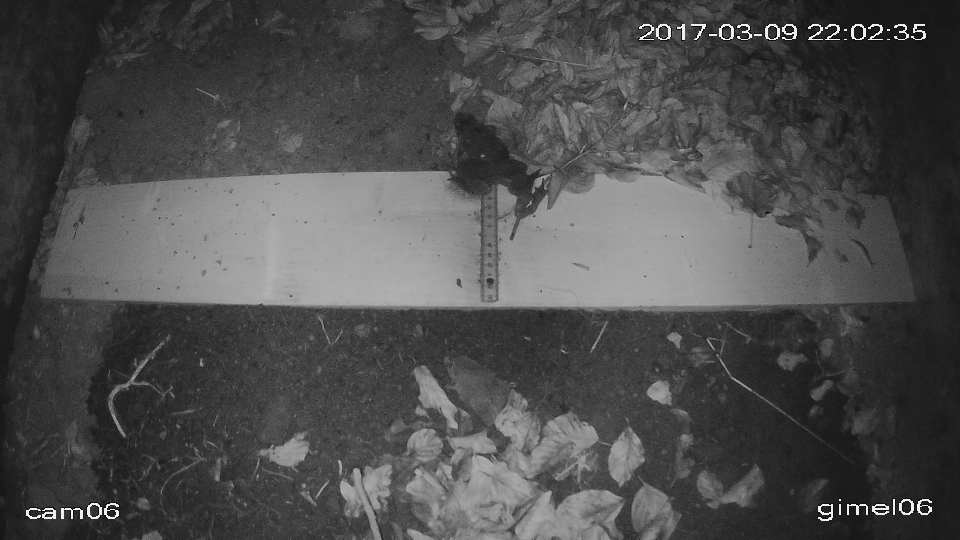
\includegraphics[width=0.9\textwidth]{images/failed_pred5_retina_big.png}
        \caption{Non détection du crapaud}
        \label{fig:eval_retina_b}
    \end{subfigure}
    \begin{subfigure}[h]{0.7\textwidth}
        \centering
        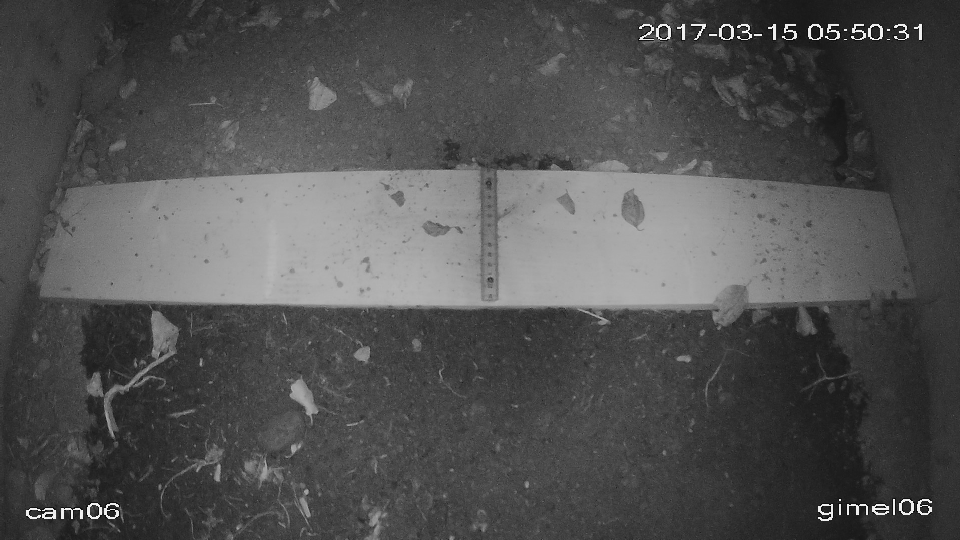
\includegraphics[width=0.9\linewidth]{images/failed_pred4_retina.png}
        \caption{Animal non détecté}
        \label{fig:eval_retina_c}
    \end{subfigure}
    \caption{Exemple d'images mal prédites par RetinaNet}
    \label{fig:failed_pred_retina}
\end{figure}
Nous pouvons voir dans la figure \ref{fig:failed_pred_retina} que RetinaNet ne détecte jamais les tritons ce qui confirme les scores du benchmark COCO vu précédement. Nous avons pensé que c'était du à la petite taille de ces derniers, cependant nous pouvons observé que l'image \ref{fig:eval_retina_b} est un gros crapaud qui n'est pas non plus reconnu. Il faut remarquer que du set de test, il s'agit de l'unique occurence d'une telle erreur.
On peut noter que les crapauds-grenouilles sont toujours très bien détectés par RetinaNet. L'image \ref{fig:eval_retina_c} nous montre un problème similaire à celui vu prédécement sur l'image \ref{fig:eval_fasterRCNN_a} ce qui tend à confirmer l'hypothèse du manque de lumière sur les cotés.
\paragraph{}
 Après avoir regardé toutes les prédictions sur les images du set de test pour les deux modèles nous avons remarqué que plusieurs images semblent provenir de la même séquence, ainsi lorsque la détection ne fontionne pas, elle ne fonctionne pas plusieurs fois! Ceci implique que les erreurs sont comptabilisées à double, cependant nous ne pouvons pas crier victoire et dire que nos scores sont bien en dessous de leur vrai valeurs car nous observons aussi ceci sur les prédictions correctes! Ainsi les bons scores et mauvais scores à double se compensent.

 \paragraph{Conclusion} Nos deux modèles semblent avoir des difficultés avec les animaux qui passent par les cotés, il se peut, au vu des nombreuses annotations d'entrainement placées au centre de l'image, que les modèles détectent mieux les animaux au centre de l'image de part leur entrainement. Néanmoins, un ajustement de la luminosité serait une piste de réflexion.

\chapter{Deployment}

\section{Section1}
\paragraph{paragraph1}
\subsection{Features}


\chapter{Conclusion}
Ceci est un acronyme \acl{kNN}

\end{document}
